\documentclass[11pt,a4paper]{article}
\usepackage[a4paper,top=26mm,bottom=24mm,left=25mm,right=25mm,headheight=23pt]{geometry}
\usepackage{amsmath,amssymb,amsthm,mathtools}
\usepackage{booktabs,array,tabularx}
\usepackage{enumitem}
\usepackage{xcolor,graphicx}
\usepackage{tikz}
\usetikzlibrary{arrows.meta,calc,positioning}
\usepackage{microtype}
\usepackage{fancyhdr,titlesec}
\usepackage[colorlinks=true,linkcolor=teal!45!black,urlcolor=teal!45!black,
  pdftitle={MTL781 Post-Minor Lecture Notes},
  pdfsubject={Finite Element Theory and Applications}]{hyperref}

\definecolor{Heading}{HTML}{133844}
\definecolor{Muted}{HTML}{4F626A}
\definecolor{Rule}{HTML}{B8CFD0}
\definecolor{Tint}{HTML}{EDF5F4}
\setcounter{secnumdepth}{0}
\setcounter{tocdepth}{1}
\setlength{\parindent}{0pt}
\setlength{\emergencystretch}{1.25em}
\setlength{\parskip}{0.48em plus 0.15em minus 0.08em}
\setlength{\fboxsep}{8pt}
\setlist{topsep=0.3em,itemsep=0.14em,parsep=0.14em}
\titleformat{\section}{\sffamily\bfseries\Large\color{Heading}}{}{0pt}{}
\titleformat{\subsection}{\sffamily\bfseries\large\color{Heading}}{}{0pt}{}
\titleformat{\subsubsection}{\sffamily\bfseries\normalsize\color{Heading}}{}{0pt}{}
\titlespacing*{\section}{0pt}{0pt}{0.8em}
\titlespacing*{\subsection}{0pt}{1.25em}{0.3em}
\titlespacing*{\subsubsection}{0pt}{0.9em}{0.2em}
\renewcommand{\contentsname}{Contents}
\renewcommand{\arraystretch}{1.13}
\allowdisplaybreaks[2]
\raggedbottom

\pagestyle{fancy}
\fancyhf{}
\fancyhead[L]{\small\sffamily\color{Muted}MTL781}
\fancyhead[R]{\small\sffamily\color{Muted}Post-minor lecture notes}
\fancyfoot[R]{\small\sffamily\color{Muted}\thepage}
\renewcommand{\headrulewidth}{0.45pt}
\renewcommand{\headrule}{\hbox to\headwidth{\color{Rule}\leaders\hrule height \headrulewidth\hfill}}

\newcommand{\lecturesource}[1]{%
  \par{\small\sffamily\color{Muted}#1}\par\vspace{0.15em}}
\newcommand{\editorialnote}[1]{%
  \par\noindent\colorbox{Tint}{\parbox{\dimexpr\linewidth-2\fboxsep\relax}{#1}}\par}
\begin{document}
\thispagestyle{fancy}
\vspace*{0.65em}
{\sffamily\bfseries\color{Muted} MTL781\par}
{\sffamily\bfseries\huge\color{Heading} Finite Element Theory\\[0.14em] and Applications\par}
\vspace{0.45em}
{\sffamily\large\color{Muted} Post-minor lecture notes \quad\textbullet\quad Lectures 6--15\par}
\vspace{0.9em}
{\color{Rule}\rule{\textwidth}{0.75pt}}\par
\vspace{0.45em}
Typed from the handwritten post-minor PDFs. The notes retain the lecture order,
proofs, examples, and exercises. Source page numbers refer to the original PDFs.
Inline notes explain substantive corrections and added derivation steps.

\editorialnote{\textbf{Lecture 12 is reconstructed.} Its handwritten notes were
missing. The reconstruction uses the end of Lecture 11 and the material
marked \emph{Recall} at the start of Lecture 13.}

\vspace{1.15em}
\tableofcontents

\clearpage
\section{Lecture 6. The weak Dirichlet problem and the trace theorem}
\lecturesource{Source \enspace\texttt{Lec6\_annotated.pdf}, pp.~1--9}

% Source pages 1--2 and first line of page 3.
\subsection{Bilinear forms and the Lax--Milgram lemma}

Let \(V\) be a real Hilbert space with norm \(\|\cdot\|_V\). A
bilinear form \(a\colon V\times V\to\mathbb R\) is linear in each
argument when the other is fixed. Thus
\begin{align*}
a(\alpha_1u_1+\alpha_2u_2,w)
  &=\alpha_1a(u_1,w)+\alpha_2a(u_2,w),\\
a(u,\beta_1w_1+\beta_2w_2)
  &=\beta_1a(u,w_1)+\beta_2a(u,w_2).
\end{align*}
The form is \emph{bounded} or \emph{continuous} if some \(M>0\)
satisfies
\[
  |a(v,w)|\le M\|v\|_V\|w\|_V
  \qquad (v,w\in V).
\]
It is \emph{coercive} or \emph{\(V\)-elliptic} if some
\(\alpha>0\) satisfies
\[
  a(w,w)\ge\alpha\|w\|_V^2
  \qquad (w\in V).
\]

For example, take \(V=H^1(\Omega)\) and
\[
  a(v,w)=\int_\Omega \nabla v\cdot\nabla w\,dx+\int_\Omega vw\,dx,
  \qquad
  \|v\|_{H^1(\Omega)}^2=\|v\|_{L^2(\Omega)}^2+
                             \|\nabla v\|_{L^2(\Omega)}^2.
\]
Apply Cauchy--Schwarz to each integral and then to the two pairs
of nonnegative norms. With all \(L^2\) norms below taken over \(\Omega\),
\begin{align*}
  |a(v,w)|
  &\le \|\nabla v\|_{L^2}\|\nabla w\|_{L^2}
     +\|v\|_{L^2}\|w\|_{L^2}\\
  &\le
  \bigl(\|\nabla v\|_{L^2}^2+\|v\|_{L^2}^2\bigr)^{1/2}
  \bigl(\|\nabla w\|_{L^2}^2+\|w\|_{L^2}^2\bigr)^{1/2}\\
  &=\|v\|_{H^1(\Omega)}\|w\|_{H^1(\Omega)}.
\end{align*}
Also \(a(v,v)=\|v\|_{H^1(\Omega)}^2\). The continuity and
coercivity constants can both be chosen equal to one.

\medskip
\noindent\textbf{Lax--Milgram lemma.}
If \(a\) is a bounded, coercive bilinear form on a real Hilbert
space \(V\) and \(L\colon V\to\mathbb R\) is a bounded linear
functional, there exists a unique \(u\in V\) such that
\[
  a(u,v)=L(v)\qquad \text{for all }v\in V.
\]

% Source pages 3--4 and first half of page 5.
\subsection{Homogeneous Dirichlet problem}

Let \(\Omega\subset\mathbb R^2\) be a bounded open domain. The
homogeneous Dirichlet problem for the Poisson equation is
\[
  -\Delta u=f\quad\text{in }\Omega,\qquad
  u=0\quad\text{on }\partial\Omega,\qquad
  \Delta=\frac{\partial^2}{\partial x_1^2}
         +\frac{\partial^2}{\partial x_2^2}.
\]
In one dimension, on \(\Omega=(a,b)\), the corresponding problem
is \(-u''(x)=f(x)\) for \(a<x<b\), with \(u(a)=u(b)=0\).
A classical solution belongs to \(C^2(\Omega)\cap C(\overline\Omega)\)
and satisfies the equation and boundary condition pointwise.

Set \(\mathcal D(\Omega)=C_c^\infty(\Omega)\).
Multiply the equation by \(v\in\mathcal D(\Omega)\) and integrate.
Green's identity gives
\[
  -\int_\Omega \Delta u\,v\,dx
  =\int_\Omega \nabla u\cdot\nabla v\,dx
  =\int_\Omega f v\,dx.
\]
The boundary contribution vanishes because \(v\) is compactly
supported in \(\Omega\). With \(u\in H_0^1(\Omega)\),
density of \(\mathcal D(\Omega)\) and continuity of both
integrals extend the equation to all \(v\in H_0^1(\Omega)\).
Here \(H_0^1(\Omega)\) is the \(H^1\)-closure of \(\mathcal D(\Omega)\).
On a domain admitting a trace, its elements have zero boundary trace.

\medskip
\noindent\textbf{Weak formulation.}
Given \(f\in L^2(\Omega)\), find the weak solution \(u\) in the
trial space \(H_0^1(\Omega)\) satisfying
\begin{equation}
  \int_\Omega\nabla u\cdot\nabla v\,dx=\int_\Omega f v\,dx
  \qquad\text{for all test functions }v\in H_0^1(\Omega).
  \label{eq:l6-dirichlet-weak}
\end{equation}
The test space is also \(H_0^1(\Omega)\). In variational notation
the two sides are \(a(u,v)\) and \(L(v)\), respectively. To apply
Lax--Milgram, Cauchy--Schwarz gives
\[
  |a(w,v)|\le \|w\|_{H^1(\Omega)}\|v\|_{H^1(\Omega)},\qquad
  |L(v)|\le \|f\|_{L^2(\Omega)}\|v\|_{H^1(\Omega)}.
\]
The Poincar\'e inequality on \(H_0^1(\Omega)\) gives
\(\|v\|_{L^2(\Omega)}\le C_P\|\nabla v\|_{L^2(\Omega)}\).
Consequently
\[
  a(v,v)=|v|_{H^1(\Omega)}^2
         =\|\nabla v\|_{L^2(\Omega)}^2
  \ge (1+C_P^2)^{-1}\|v\|_{H^1(\Omega)}^2 .
\]
There exists a unique weak solution by Lax--Milgram.

Taking \(v=u\) in \eqref{eq:l6-dirichlet-weak} gives
\begin{align*}
  |u|_{H^1(\Omega)}^2
  &=\int_\Omega fu\,dx\\
  &\le \|f\|_{L^2(\Omega)}\|u\|_{L^2(\Omega)}
  \le C_P\|f\|_{L^2(\Omega)}|u|_{H^1(\Omega)}.
\end{align*}
It follows that \(|u|_{H^1(\Omega)}\le C_P\|f\|_{L^2(\Omega)}\),
with the zero-seminorm case included directly. Another use
of Poincar\'e gives a bound in the full norm.
\[
  \|u\|_{H^1(\Omega)}
  \le \sqrt{1+C_P^2}\,|u|_{H^1(\Omega)}
  \le C\|f\|_{L^2(\Omega)}.
\]
Applying this estimate to the difference of any two solutions gives
continuous dependence on the data. Existence, uniqueness and
continuous dependence are the three criteria for well-posedness in
the sense of Hadamard.

% Source remainder of page 5 and page 6.
\subsection{Energy minimization and classical solutions}

The form for \eqref{eq:l6-dirichlet-weak} is symmetric, since
\(\nabla v\cdot\nabla w=\nabla w\cdot\nabla v\).
The solution is the unique minimizer over \(H_0^1(\Omega)\) of
\[
  J(v)=\tfrac12 a(v,v)-L(v)
      =\tfrac12\int_\Omega|\nabla v|^2\,dx-\int_\Omega fv\,dx .
\]
Indeed, the directional derivative satisfies
\[
  J'(u)[v]=a(u,v)-L(v).
\]
At a minimizer all directions \(v\in H_0^1(\Omega)\) give zero
derivative. This is the Euler--Lagrange equation in
\eqref{eq:l6-dirichlet-weak}, analogous to \(F'(x)=0\) at an
interior minimum of a differentiable real function.
Conversely, if \(J'(u)[v]=0\) for all \(v\), then
\[
  J(u+v)-J(u)=\tfrac12 a(v,v)\ge 0.
\]
Coercivity makes the inequality strict for \(v\ne 0\).

A classical solution in the energy space \(H_0^1(\Omega)\) is a
weak solution by the derivation above. Conversely, suppose that
the weak solution \(u\) also lies in
\(C^2(\Omega)\cap C(\overline\Omega)\) and that
\(f\in C(\overline\Omega)\). For \(v\in\mathcal D(\Omega)\),
integration by parts in \eqref{eq:l6-dirichlet-weak} yields
\[
  \int_\Omega(-\Delta u-f)v\,dx=0 .
\]
The residual is zero as a distribution and hence is zero almost
everywhere. Its continuity gives \(-\Delta u=f\) pointwise in
\(\Omega\). On a domain with the trace property, the zero trace
and continuity of \(u\) up to the boundary give \(u=0\) there.

\smallskip
\noindent\emph{Proof detail.}
The handwritten proof tests the last identity directly with the
residual \(-\Delta u-f\). A residual in \(L^2(\Omega)\) can be
tested by approximating it by members of \(\mathcal D(\Omega)\)
in \(L^2\). This yields \(\int_\Omega(-\Delta u-f)^2\,dx=0\).
The distribution argument above also works with an interior
continuous residual that is only locally integrable.

There are two steps in obtaining this extra regularity.
Elliptic regularity gives a gain of two Sobolev derivatives,
\(f\in H^m(\Omega)\) implies \(u\in H^{m+2}(\Omega)\) for the
homogeneous Dirichlet problem under suitable boundary smoothness,
where \(m\) is a nonnegative integer.
Sobolev embedding then gives classical differentiability if
\(m+2>k+n/2\) for \(C^k\) regularity in dimension \(n\), under
the corresponding domain assumptions. In the two-dimensional
examples, \(H^2\) embeds into \(C^0\) and \(H^3\) embeds into
\(C^1\) on a bounded domain with a Sobolev extension property.
More generally, the analogous \(W^{s,p}\) embedding into \(C^k\)
holds when \(s>k+n/p\), for suitable domains.

% Source page 7.
\subsection{Boundary conditions for elliptic problems}

Write \(\partial_\nu u=\nabla u\cdot\nu\) for the outward
normal derivative.

\begin{enumerate}
  \item \textbf{Dirichlet.}
    In the Poisson problem \(-\Delta u=f\) one prescribes
    \(u=0\) on \(\partial\Omega\) for homogeneous data and
    \(u=g\) on \(\partial\Omega\) for nonhomogeneous data.
    The lecture also lists \(-\Delta u+u=f\) with
    \(u=0\) on \(\partial\Omega\) as a homogeneous example.
  \item \textbf{Neumann.}
    The example is \(-\Delta u+u=f\) in \(\Omega\) with
    \(\partial_\nu u=g\) on \(\partial\Omega\). The condition is
    homogeneous when \(g=0\). On \((a,b)\) the homogeneous
    example is \(-u''+u=f\) with \(u'(a)=u'(b)=0\).
  \item \textbf{Robin.}
    The example is \(-\Delta u=f\) in \(\Omega\) with
    \(\partial_\nu u+\alpha u=0\) on \(\partial\Omega\).
    An interval example with the lower-order term is
    \[
      -u''+u=f,\qquad
      -u'(a)+\alpha_1u(a)=0,\qquad
      u'(b)+\alpha_2u(b)=0 .
    \]
    The signs and endpoints in the interval conditions follow
    from the outward normals \(\nu(a)=-1\) and \(\nu(b)=1\).
    This corrects crossed endpoints in the handwritten
    Robin example.
  \item \textbf{Mixed.}
    For \(\partial\Omega=\overline{\Gamma_1}\cup
    \overline{\Gamma_2}\), with the two relatively open pieces
    disjoint, the example is
    \[
      -\Delta u+u=f\quad\text{in }\Omega,\qquad
      u=0\text{ on }\Gamma_1,\qquad
      \partial_\nu u=0\text{ on }\Gamma_2 .
    \]
    On \((a,b)\) this gives \(-u''+u=f\) with \(u(a)=0\)
    and \(u'(b)=0\). The interval equations for Robin and mixed
    data use the sign of \(-\Delta\) from the displayed PDEs.
\end{enumerate}

\begin{center}
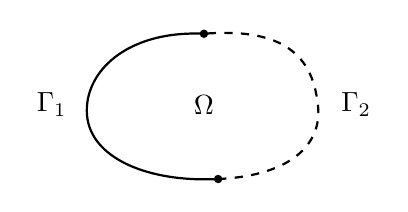
\begin{tikzpicture}[scale=0.9]
  \draw[thick]
    (0,1.15) .. controls (-1.1,1.2) and (-1.7,0.6) .. (-1.65,0)
             .. controls (-1.6,-0.6) and (-0.8,-0.95) .. (0.2,-0.9);
  \draw[thick,dashed]
    (0.2,-0.9) .. controls (1.3,-0.85) and (1.7,-0.35) .. (1.6,0.2)
              .. controls (1.5,1.0) and (0.9,1.22) .. (0,1.15);
  \fill (0,1.15) circle (1.7pt) (0.2,-0.9) circle (1.7pt);
  \node at (0,0.15) {\(\Omega\)};
  \node[left] at (-1.8,0.15) {\(\Gamma_1\)};
  \node[right] at (1.8,0.15) {\(\Gamma_2\)};
\end{tikzpicture}
\end{center}

% Source pages 8--9.
\subsection{Values at the boundary and the trace theorem}

For nonhomogeneous Dirichlet data, the prescribed equation is
\(-\Delta u=f\) in \(\Omega\) with \(u=g\) on \(\partial\Omega\).
Boundary values require a separate interpretation for Sobolev
functions. For example, on \([0,1]\), let \(f_1(x)=1\) everywhere
and put
\[
  f_2(x)=
  \begin{cases}
    1, & 0<x<1,\\
    0, & x=0,\\
    1500, & x=1.
  \end{cases}
\]
The overwritten value at \(x=0\) is read here as zero.
Changing the endpoint values leaves the \(L^2(0,1)\) element
and integral unchanged, so
\(\int_0^1 f_1(x)\,dx=\int_0^1 f_2(x)\,dx=1\).
The notation \(v=0\) on \(\partial\Omega\) for \(v\in H^1(\Omega)\)
refers to its trace. The pointwise interpretation applies when
\(v\) is continuous up to the boundary.

By the definition of \(H_0^1(\Omega)\), each
\(\phi\in H_0^1(\Omega)\) has approximants
\(\phi_m\in\mathcal D(\Omega)\) with
\(\phi_m\to\phi\) in \(H^1(\Omega)\).
On a bounded domain with \(C^1\) boundary, each
\(\phi\in H^1(\Omega)\) can be approximated in \(H^1(\Omega)\)
by \(\phi_m\in C^\infty(\overline\Omega)\), meaning smooth up
to the boundary. The smooth approximants define the trace
by
\[
  \phi|_{\partial\Omega}
  =\lim_{m\to\infty}\phi_m|_{\partial\Omega}
  \quad\text{in }L^2(\partial\Omega).
\]
Continuity of the trace makes this limit independent of the
approximating sequence.

\begin{center}
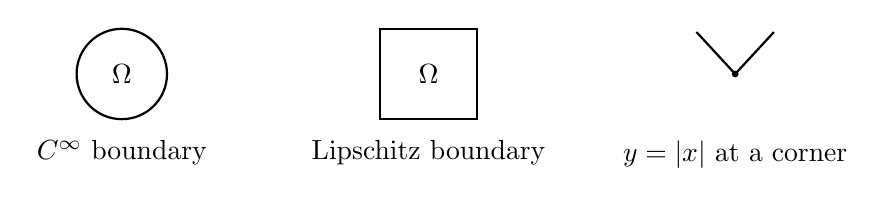
\begin{tikzpicture}[scale=0.82]
  \draw[thick] (0,0) circle (0.7);
  \node at (0,0) {\(\Omega\)};
  \node[below] at (0,-0.88) {\(C^\infty\) boundary};
  \draw[thick] (4.0,-0.7) rectangle (5.5,0.7);
  \node at (4.75,0) {\(\Omega\)};
  \node[below] at (4.75,-0.88) {Lipschitz boundary};
  \draw[thick] (8.9,0.65)--(9.5,0)--(10.1,0.65);
  \fill (9.5,0) circle (1.5pt);
  \node[below] at (9.5,-0.88) {\(y=|x|\) at a corner};
\end{tikzpicture}
\end{center}

The disk illustrates smooth boundary. The square has Lipschitz
boundary, and after rotation its corner is locally modeled by the
graph of \(|x|\), which is Lipschitz and fails to be \(C^1\) at zero.
The trace conclusions also hold on bounded Lipschitz domains.

\medskip
\noindent\textbf{Trace theorem.}
For a bounded domain \(\Omega\subset\mathbb R^n\), \(n\ge 1\),
with \(C^1\) boundary, there is a continuous linear map
\[
  \gamma\colon H^1(\Omega)\longrightarrow L^2(\partial\Omega),
  \qquad
  \gamma(v)=v|_{\partial\Omega}\quad
  \text{if }v\in H^1(\Omega)\cap C(\overline\Omega).
\]
The trace operator \(\gamma\) has
\begin{align*}
  \ker\gamma
    &=\{v\in H^1(\Omega):\gamma(v)=0\}=H_0^1(\Omega),\\
  \operatorname{ran}\gamma&=H^{1/2}(\partial\Omega).
\end{align*}
Thus every \(g\in H^{1/2}(\partial\Omega)\) has a lift
\(v\in H^1(\Omega)\) with \(\gamma(v)=g\).

\clearpage
\section{Lecture 7. Nonhomogeneous Dirichlet and Neumann problems}
\lecturesource{Source \enspace\texttt{Lec7\_annotated.pdf}, pp.~1--11}

% Source page 1, trace recall.
\subsection{The trace map}

On a bounded domain with the boundary regularity of the trace
theorem, the continuous linear trace map
\(\gamma\colon H^1(\Omega)\to L^2(\partial\Omega)\) satisfies
\[
  \|\gamma(v)\|_{L^2(\partial\Omega)}
  \le C_{\mathrm{tr}}\|v\|_{H^1(\Omega)},\qquad
  \ker\gamma=H_0^1(\Omega),\qquad
  \operatorname{ran}\gamma=H^{1/2}(\partial\Omega).
\]
For \(v\) continuous up to the boundary, \(\gamma(v)\) is the restriction
\(v|_{\partial\Omega}\). In general the notation \(v=0\) on
\(\partial\Omega\) means \(\gamma(v)=0\). Every
\(h\in H^{1/2}(\partial\Omega)\) has at least one lift
\(v\in H^1(\Omega)\) satisfying \(\gamma(v)=h\).

% Source pages 1--4.
\subsection{Nonhomogeneous Dirichlet data}

Consider
\[
  -\Delta u=f\quad\text{in }\Omega,\qquad
  u=g\quad\text{on }\partial\Omega.
\]
For \(\Omega=(a,b)\), this reads \(-u''(x)=f(x)\) in \((a,b)\)
with \(u(a)=\alpha_1\) and \(u(b)=\alpha_2\).
The multidimensional classical solution is sought in
\(C^2(\Omega)\cap C(\overline\Omega)\).

For the weak problem let \(f\in L^2(\Omega)\) and
\(g\in H^{1/2}(\partial\Omega)\). Choose a lift
\(\widetilde u\in H^1(\Omega)\) with \(\gamma(\widetilde u)=g\).
Set \(w=u-\widetilde u\), so \(w\in H_0^1(\Omega)\). The set
of admissible \(u\) is
\[
  K=\{z\in H^1(\Omega):z-\widetilde u\in H_0^1(\Omega)\}
   =\{z\in H^1(\Omega):\gamma(z)=g\}.
\]
It is the translate \(\widetilde u+H_0^1(\Omega)\), and the
test space is \(H_0^1(\Omega)\).

For smooth functions the shifted equation is
\[
  -\Delta w=-\Delta(u-\widetilde u)
           =f+\Delta\widetilde u,\qquad w=0\text{ on }\partial\Omega.
\]
The same interior identity holds in the sense of distributions
for an \(H^1\) lift. The intermediate expansion in the
handwritten calculation has its sign reversed on
\(\Delta\widetilde u\). The final shifted equation uses the plus sign shown here.

Define
\[
  a(z,v)=\int_\Omega \nabla z\cdot\nabla v\,dx,\qquad
  L(v)=\int_\Omega f v\,dx-\int_\Omega\nabla\widetilde u\cdot\nabla v\,dx .
\]
The shifted weak problem is to find \(w\in H_0^1(\Omega)\)
with \(a(w,v)=L(v)\) for every \(v\in H_0^1(\Omega)\).
The signed term \(-\int_\Omega\nabla\widetilde u\cdot\nabla v\,dx\)
is the action of \(\Delta\widetilde u\) on the test space.
This formula makes sense for any \(H^1\) lift.

For \(z,v\in H_0^1(\Omega)\), Cauchy--Schwarz and Poincar\'e
give
\[
  |a(z,v)|\le\|z\|_{H^1(\Omega)}\|v\|_{H^1(\Omega)},\qquad
  a(v,v)=|v|_{H^1(\Omega)}^2\ge\alpha\|v\|_{H^1(\Omega)}^2 .
\]
Here \(\alpha>0\) depends on the Poincar\'e constant. The
functional \(L\) is linear and
\begin{align*}
  |L(v)|
  &\le\left|\int_\Omega f v\,dx\right|+
       \left|\int_\Omega\nabla\widetilde u\cdot\nabla v\,dx\right|\\
  &\le\|f\|_{L^2(\Omega)}\|v\|_{L^2(\Omega)}
        +\|\nabla\widetilde u\|_{L^2(\Omega)}
         \|\nabla v\|_{L^2(\Omega)}\\
  &\le\bigl(\|f\|_{L^2(\Omega)}
        +\|\nabla\widetilde u\|_{L^2(\Omega)}\bigr)\|v\|_{H^1(\Omega)} .
\end{align*}
Thus \(L\in(H_0^1(\Omega))^*\), and Lax--Milgram gives a unique
\(w\) solving the shifted equation. Adding the lift gives
\(u=w+\widetilde u\in K\), which satisfies
\begin{equation}
  \int_\Omega \nabla u\cdot\nabla v\,dx
    =\int_\Omega f v\,dx\qquad(v\in H_0^1(\Omega)).
  \label{eq:l7-dirichlet-weak}
\end{equation}
This is the weak formulation in the original variable.

For uniqueness directly in \(K\), suppose \(u_1,u_2\in K\) solve
\eqref{eq:l7-dirichlet-weak}. Subtract their equations and take
\(v=u_1-u_2\in H_0^1(\Omega)\). Then
\[
  \int_\Omega|\nabla(u_1-u_2)|^2\,dx=0,\qquad
  \|u_1-u_2\|_{L^2(\Omega)}
    \le C_P\|\nabla(u_1-u_2)\|_{L^2(\Omega)}=0 .
\]
Hence \(u_1=u_2\) almost everywhere. In particular the physical
solution is independent of which lift was chosen.

Testing the shifted equation with \(w\) and using coercivity gives
\[
  \|w\|_{H^1(\Omega)}
    \le C\bigl(\|f\|_{L^2(\Omega)}+\|\widetilde u\|_{H^1(\Omega)}\bigr).
\]
The trace theorem, with target \(H^{1/2}(\partial\Omega)\),
allows a lift satisfying
\[
  \|\widetilde u\|_{H^1(\Omega)}
    \le C\|g\|_{H^{1/2}(\partial\Omega)}.
\]
This lift bound follows from the open mapping theorem
applied to the bounded, surjective trace map onto that target.
The triangle inequality gives the estimate recorded in the
lecture,
\[
  \|u\|_{H^1(\Omega)}
   \le C\bigl(\|f\|_{L^2(\Omega)}
              +\|g\|_{H^{1/2}(\partial\Omega)}\bigr).
\]
Apply the same estimate to differences to obtain continuous
dependence on \(f\) and \(g\), completing well-posedness.
If \(u\) additionally belongs to \(C^2(\Omega)\cap
C(\overline\Omega)\) and the data have continuous
representatives, compactly supported tests recover the pointwise
PDE and the trace gives the classical boundary value.

% Source pages 5--8, through the first Neumann proof.
\subsection{Homogeneous Neumann data}

For a bounded open domain \(\Omega\subset\mathbb R^2\), take
\[
  -\Delta u+u=f\quad\text{in }\Omega,\qquad
  \partial_\nu u=0\quad\text{on }\partial\Omega ,
\]
with \(\partial_\nu u=\nabla u\cdot\nu\) the outward normal
derivative. An example is \(\Omega=(0,1)\times(0,1)\).

\begin{center}
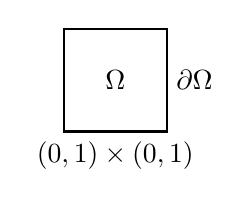
\begin{tikzpicture}[scale=0.9]
  \draw[thick] (0,0) rectangle (1.45,1.45);
  \node at (0.725,0.725) {\(\Omega\)};
  \node[right] at (1.45,0.725) {\(\partial\Omega\)};
  \node[below] at (0.725,0) {\((0,1)\times(0,1)\)};
\end{tikzpicture}
\end{center}

In the lecture's interval notation the problem
\(-u''+u=f\) on \((a,b)\) has derivative data
\(u'(a)=\alpha_1,\ u'(b)=\alpha_2\).
Homogeneous data mean \(\alpha_1=\alpha_2=0\).
If the data are expressed as outward normal derivatives, their
values at the two endpoints are \(-\alpha_1\) and \(\alpha_2\).

Assume first that \(u\in C^2(\overline\Omega)\) is a classical
solution. Multiply the PDE by \(v\in C^\infty(\overline\Omega)\),
integrate and apply Green's identity to the Laplacian term.
\[
  -\int_\Omega\Delta u\,v\,dx
  =\int_\Omega\nabla u\cdot\nabla v\,dx
     -\int_{\partial\Omega}(\partial_\nu u)v\,ds.
\]
The boundary integral is zero by the prescribed Neumann
condition. Smooth functions up to the boundary are dense
in \(H^1(\Omega)\) on the domains under consideration.
The weak formulation for \(f\in L^2(\Omega)\) is to find
\(u\in H^1(\Omega)\) such that
\begin{equation}
  \int_\Omega\nabla u\cdot\nabla v\,dx+\int_\Omega uv\,dx
  =\int_\Omega f v\,dx\qquad(v\in H^1(\Omega)).
  \label{eq:l7-neumann-zero}
\end{equation}
Both the trial and test spaces are the full \(H^1(\Omega)\).

To apply Lax--Milgram, write \(a(w,v)\) for the left-hand
bilinear form, with first argument \(w\), and put
\(L(v)=\int_\Omega f v\,dx\). Cauchy--Schwarz in the integrals
and then in \(\mathbb R^2\) gives
\begin{align*}
  |a(w,v)|
  &\le\|\nabla w\|_{L^2(\Omega)}\|\nabla v\|_{L^2(\Omega)}
      +\|w\|_{L^2(\Omega)}\|v\|_{L^2(\Omega)}\\
  &\le\|w\|_{H^1(\Omega)}\|v\|_{H^1(\Omega)},\\
  a(v,v)&=\|\nabla v\|_{L^2(\Omega)}^2+\|v\|_{L^2(\Omega)}^2
         =\|v\|_{H^1(\Omega)}^2 .
\end{align*}
Also
\[
  |L(v)|\le\|f\|_{L^2(\Omega)}\|v\|_{L^2(\Omega)}
          \le\|f\|_{L^2(\Omega)}\|v\|_{H^1(\Omega)}.
\]
There is a unique \(u\in H^1(\Omega)\) satisfying
\eqref{eq:l7-neumann-zero}. Taking \(v=u\) gives
\[
  \|u\|_{H^1(\Omega)}^2=\int_\Omega f u\,dx
      \le \|f\|_{L^2(\Omega)}\|u\|_{H^1(\Omega)},
  \qquad
  \|u\|_{H^1(\Omega)}\le\|f\|_{L^2(\Omega)}.
\]
As in the Dirichlet case, the estimate implies continuous
dependence on the data and hence well-posedness.

To recover the PDE for a smooth weak solution, take
\(v\in\mathcal D(\Omega)\) in \eqref{eq:l7-neumann-zero} and
integrate by parts. The identity
\(\int_\Omega(-\Delta u+u-f)v\,dx=0\) gives
\(-\Delta u+u=f\) almost everywhere, and pointwise when
\(f\) is continuous. Green's identity with general \(H^1\)
tests now gives
\[
  \int_{\partial\Omega}(\partial_\nu u)\gamma(v)\,ds=0
    \qquad(v\in H^1(\Omega)).
\]
The traces \(H^{1/2}(\partial\Omega)\) are dense in
\(L^2(\partial\Omega)\). Thus \(\partial_\nu u=0\) as an
\(L^2\) boundary function, so the solution satisfies the
classical condition where the normal derivative is continuous.
On a smooth domain, the same boundary argument applies to
\(u\in H^2(\Omega)\) using the outward normal component of
the trace of \(\nabla u\). More precisely, the handwritten choice of
\(v=\partial_\nu u\) means using an interior test with the
specified \emph{trace} when such a lift is available. Density
of traces is sufficient when the normal derivative is in \(L^2\).

% Source pages 8--10, through the classical-solution remark.
\subsection{Nonhomogeneous Neumann data}

Consider
\[
  -\Delta u+u=f\quad\text{in }\Omega,\qquad
  \partial_\nu u=g\quad\text{on }\partial\Omega.
\]
For a smooth solution and a smooth test \(v\), multiply
the PDE by \(v\), integrate, and replace
\(-\int_\Omega \Delta u\,v\,dx\) using
\[
  -\int_\Omega\Delta u\,v\,dx
   =\int_\Omega\nabla u\cdot\nabla v\,dx
      -\int_{\partial\Omega}g v\,ds .
\]
Moving the last integral to the right gives a positive
Neumann load. For \(f\in L^2(\Omega)\) and
\(g\in L^2(\partial\Omega)\), the weak problem is to find
\(u\in H^1(\Omega)\) with
\begin{equation}
  \int_\Omega\nabla u\cdot\nabla v\,dx+\int_\Omega uv\,dx
  =\int_\Omega f v\,dx+\int_{\partial\Omega}g\gamma(v)\,ds
  \qquad(v\in H^1(\Omega)).
  \label{eq:l7-neumann-data}
\end{equation}
The trace makes the boundary integral continuous, so the
identity derived with smooth tests extends to \(H^1(\Omega)\)
by density.

The left-hand form is continuous and \(H^1(\Omega)\)-elliptic
as before. The right-hand functional \(L\) is linear, and
Cauchy--Schwarz followed by the trace estimate gives
\begin{align*}
  |L(v)|
  &\le\|f\|_{L^2(\Omega)}\|v\|_{L^2(\Omega)}
      +\|g\|_{L^2(\partial\Omega)}\|\gamma(v)\|_{L^2(\partial\Omega)}\\
  &\le\bigl(\|f\|_{L^2(\Omega)}
              +C_{\mathrm{tr}}\|g\|_{L^2(\partial\Omega)}\bigr)
       \|v\|_{H^1(\Omega)} .
\end{align*}
By Lax--Milgram, there is a unique weak solution. Setting \(v=u\)
gives
\[
  \|u\|_{H^1(\Omega)}
  \le C\bigl(\|f\|_{L^2(\Omega)}
             +\|g\|_{L^2(\partial\Omega)}\bigr).
\]
The problem is well-posed. If the solution is in
\(C^2(\overline\Omega)\cap H^1(\Omega)\), compactly supported
tests recover \(-\Delta u+u=f\) and the remaining boundary
identity is
\[
  \int_{\partial\Omega}(\partial_\nu u-g)\gamma(v)\,ds=0
  \qquad(v\in H^1(\Omega)).
\]
This gives \(\partial_\nu u=g\) almost everywhere, and
continuous representatives give the classical solution.

% Source last portion of page 10 and page 11.
\subsection{Pure Neumann Poisson problem}

Testing \eqref{eq:l7-neumann-zero} with \(v=1\) gives
\(\int_\Omega u\,dx=\int_\Omega f\,dx\).
When the lower-order term is removed, the homogeneous
Neumann equations become
\[
  -\Delta u=f\quad\text{in }\Omega,\qquad
  \partial_\nu u=0\quad\text{on }\partial\Omega .
\]
The weak formulation asks for \(u\in H^1(\Omega)\) with
\[
  \int_\Omega\nabla u\cdot\nabla v\,dx=\int_\Omega f v\,dx
  \qquad(v\in H^1(\Omega)).
\]
The test \(v=1\) gives the compatibility condition
\(\int_\Omega f\,dx=0\). The bilinear form has
\(a(v,v)=|v|_{H^1(\Omega)}^2\), so its kernel contains
the constants and it fails to be coercive in the full
\(H^1\) space. Adding a constant to a solution preserves
the equation.

The lecture therefore imposes the normalization
\(\int_\Omega u\,dx=0\). On a connected bounded Lipschitz
domain, the Poincar\'e inequality for mean-zero functions
gives coercivity on
\[
  V=\left\{v\in H^1(\Omega):\int_\Omega v\,dx=0\right\}.
\]
For compatible \(f\), the weak solution obtained on \(V\)
also satisfies the equation for arbitrary \(H^1\) tests,
because subtracting the average of a test leaves both sides
unchanged. The normalization fixes the additive constant.
The closing headings announce Robin and mixed boundary-value
problems, whose boundary conditions were listed in Lecture 6.

\clearpage
\section{Lecture 8. Weak formulations and finite elements}
\lecturesource{Source \enspace\texttt{Lec8\_annotated.pdf}, pp.~1--14}

\subsection{Dirichlet and Neumann boundary conditions}

Let \(\Omega\subset\mathbb R^2\) be an open, bounded domain and let
\(f\in L^2(\Omega)\). Assume the boundary is regular enough for the traces and
boundary integrals below. Green's identity for smooth functions gives
\[
 \int_\Omega(-\Delta u+u)v\,dx
 =\int_\Omega\nabla u\cdot\nabla v\,dx+\int_\Omega uv\,dx
   -\int_{\partial\Omega}\partial_\nu u\,v\,ds,
\]
where \(\nu\) is the outward unit normal. The weak forms extend the resulting
volume integrals to Sobolev functions.

\paragraph{Homogeneous Dirichlet problem.}
For \(-\Delta u+u=f\) in \(\Omega\) and \(u=0\) on \(\partial\Omega\),
seek \(u\in H_0^1(\Omega)\) such that
\[
 \int_\Omega \nabla u\cdot\nabla v\,dx+\int_\Omega uv\,dx
 =\int_\Omega fv\,dx
 \qquad (v\in H_0^1(\Omega)).
\]
The trace of \(v\) vanishes, so the boundary integral drops out. The trial
space incorporates the condition on \(u\), which makes Dirichlet data an
\emph{essential boundary condition}.

\paragraph{Homogeneous Neumann problem.}
For \(-\Delta u+u=f\) in \(\Omega\) and \(\partial_\nu u=0\)
on \(\partial\Omega\), seek \(u\in H^1(\Omega)\) such that
\[
 \int_\Omega \nabla u\cdot\nabla v\,dx+\int_\Omega uv\,dx
 =\int_\Omega fv\,dx
 \qquad (v\in H^1(\Omega)).
\]
The normal derivative vanishes in the boundary term even though the test
functions have unrestricted traces. The weak form incorporates the Neumann
condition, making it a \emph{natural boundary condition}.

Both weak problems are well-posed by Lax--Milgram. The bilinear form is
continuous on \(H^1(\Omega)\) and
\(a(v,v)=\|v\|_{H^1(\Omega)}^2\). The right-hand side satisfies
\(\lvert L(v)\rvert\le\|f\|_{L^2(\Omega)}\|v\|_{H^1(\Omega)}\).
\emph{Correction.} The handwritten Neumann display drops \(\int_\Omega uv\,dx\).
The term follows from \(+u\) in the equation. The boundary contribution in
Green's identity for \(-\Delta u\) has a minus sign.

\subsection{Exercises on Robin and mixed conditions}

\paragraph{Exercise 1. Robin boundary condition.}
Write down the weak form for
\[
 -\Delta u+u=f\quad\text{in }\Omega,\qquad
 \partial_\nu u+u=0\quad\text{on }\partial\Omega,
\]
and discuss well-posedness. Substituting \(\partial_\nu u=-u\) into Green's
identity gives the weak form on \(H^1(\Omega)\)
\[
 \int_\Omega\nabla u\cdot\nabla v\,dx+\int_\Omega uv\,dx
 +\int_{\partial\Omega}uv\,ds
 =\int_\Omega fv\,dx\qquad (v\in H^1(\Omega)).
\]
The trace inequality bounds the boundary term, and its contribution to
\(a(v,v)\) is nonnegative. The two volume terms control the squared \(H^1\)
norm, so Lax--Milgram gives well-posedness.

\paragraph{Exercise 2. Mixed boundary conditions.}
Suppose \(\Gamma_1,\Gamma_2\) partition \(\partial\Omega\) up to their common
interfaces, \(\partial\Omega=\overline{\Gamma_1}\cup\overline{\Gamma_2}\)
and \(\lvert\Gamma_1\rvert>0\). Consider
\[
 -\Delta u=f\quad\text{in }\Omega,\qquad
 u=0\quad\text{on }\Gamma_1,\qquad
 \partial_\nu u=0\quad\text{on }\Gamma_2.
\]
Write down the weak form and establish its well-posedness.

\begin{center}
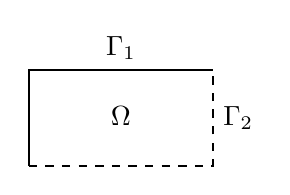
\begin{tikzpicture}[scale=.9]
 \draw[thick] (0,0)--(0,1.35)--(2.6,1.35)
   node[midway,above] {$\Gamma_1$};
 \draw[thick,dashed] (0,0)--(2.6,0)--(2.6,1.35)
   node[midway,right] {$\Gamma_2$};
 \node at (1.3,.7) {$\Omega$};
\end{tikzpicture}
\end{center}

Start with a smooth test function with \(v=0\) on \(\Gamma_1\). Then
\[
 \int_\Omega(-\Delta u)v\,dx
 =\int_\Omega\nabla u\cdot\nabla v\,dx
   -\underbrace{\int_{\Gamma_1}\partial_\nu u\,v\,ds}_{0\text{ since }v=0}
   -\underbrace{\int_{\Gamma_2}\partial_\nu u\,v\,ds}_{0\text{ since }\partial_\nu u=0}.
\]
Set \(V=\{v\in H^1(\Omega):\operatorname{Tr}v=0\text{ on }\Gamma_1\}\).
The weak problem is to find \(u\in V\) satisfying
\[
 \int_\Omega\nabla u\cdot\nabla v\,dx=\int_\Omega fv\,dx
 \qquad (v\in V).
\]
For a connected bounded Lipschitz domain, the Poincar\'e inequality on
\(V\) bounds \(\|v\|_{L^2(\Omega)}\) by \(C\|\nabla v\|_{L^2(\Omega)}\).
Consequently the gradient term is coercive on \(V\), and Lax--Milgram applies.

\paragraph{Extension to nonzero data.}
What changes when \(u=g_1\) on \(\Gamma_1\) and
\(\partial_\nu u=g_2\) on \(\Gamma_2\)? For example, if \(g_1\) admits an
\(H^1(\Omega)\) lift \(G\) and \(g_2\in L^2(\Gamma_2)\), seek \(u\in G+V\)
with
\[
 \int_\Omega\nabla u\cdot\nabla v\,dx
  =\int_\Omega fv\,dx+\int_{\Gamma_2}g_2v\,ds\qquad (v\in V).
\]
Equivalently, solve for \(w=u-G\in V\) with the additional term
\(-\int_\Omega\nabla G\cdot\nabla v\,dx\) on the right.

\subsection{Galerkin and Ritz formulations}

Starting with a boundary value problem, obtain a well-posed weak problem
on a Hilbert space \(V\). With bilinear form \(a\) and linear functional \(L\),
find \(u\in V\) such that
\[
 a(u,v)=L(v)\qquad (v\in V).
\]
For smooth solutions, the weak formulation agrees with the classical
equation and the specified boundary data. If \(a\) is symmetric and
coercive, we can characterize the weak solution by the energy
\[
 J(v)=\tfrac12 a(v,v)-L(v),\qquad J(u)=\min_{v\in V}J(v).
\]
Indeed, \(J(u+w)-J(u)=\tfrac12 a(w,w)\) for \(w\in V\) when \(u\) solves
the weak equation. Conversely, stationarity along every direction \(v\)
gives \(a(u,v)=L(v)\).

Discretize \(\Omega\) into elements \(T\). On an interval, the elements are
subintervals between consecutive nodes. In two dimensions a common choice
is a triangulation. Here are the interval and two-dimensional mesh sketches.
\begin{center}
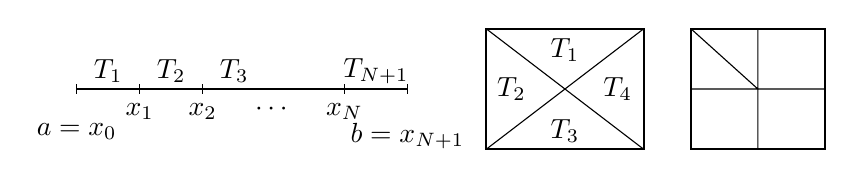
\begin{tikzpicture}[x=1cm,y=.9cm]
 \draw[thick] (0,1.2)--(4.2,1.2);
 \foreach \x/\lab in {.8/x_1,1.6/x_2,3.4/x_N}{
   \draw (\x,1.27)--(\x,1.13) node[below] {$\lab$};
 }
 \draw (0,1.27)--(0,1.13) node[below=7pt] {$a=x_0$};
 \draw (4.2,1.27)--(4.2,1.13) node[below=7pt] {$b=x_{N+1}$};
 \node at (2.5,.91) {$\cdots$};
 \node at (.4,1.45) {$T_1$};
 \node at (1.2,1.45) {$T_2$};
 \node at (2.0,1.45) {$T_3$};
 \node at (3.8,1.45) {$T_{N+1}$};
 \begin{scope}[shift={(5.2,.35)}]
  \draw[thick] (0,0) rectangle (2,1.7);
  \draw (0,0)--(2,1.7) (0,1.7)--(2,0);
  \node at (1,1.4) {$T_1$};
  \node at (.32,.85) {$T_2$};
  \node at (1,.26) {$T_3$};
  \node at (1.67,.85) {$T_4$};
 \end{scope}
 \begin{scope}[shift={(7.8,.35)}]
  \draw[thick] (0,0) rectangle (1.7,1.7);
  \draw (0,.85)--(1.7,.85) (.85,0)--(.85,1.7)
    (0,1.7)--(.85,.85);
 \end{scope}
\end{tikzpicture}
\end{center}

Choose a finite-dimensional space \(V_h\subset V\), with local
polynomial restrictions \(v_h|_T\in P_k(T)\) on each element.
The \emph{Galerkin method} finds \(u_h\in V_h\) such that
\[
 a(u_h,v_h)=L(v_h)\qquad(v_h\in V_h).
\]
The \emph{Ritz method} minimizes the energy over this same subspace,
\(J(u_h)=\min_{v_h\in V_h}J(v_h)\). For symmetric coercive \(a\),
the two procedures give the same approximation to \(u\).

For \(T\subset\mathbb R^n\), \(P_k(T)\) consists of polynomials of total
degree at most \(k\). With \(x=(x_1,\ldots,x_n)\),
\(\alpha=(\alpha_1,\ldots,\alpha_n)\in\mathbb N_0^n\)
and \(|\alpha|=\sum_{r=1}^n\alpha_r\), write
\[
 p(x)=\sum_{|\alpha|\le k}c_\alpha x_1^{\alpha_1}\cdots x_n^{\alpha_n}.
\]
In one dimension \(P_1\) consists of \(c_1+c_2x\), and \(P_2\) consists of
\(c_1+c_2x+c_3x^2\). In two dimensions the corresponding general forms are
\[
 \begin{aligned}
 p\in P_1&\quad\Longleftrightarrow\quad p(x)=c_1+c_2x_1+c_3x_2,\\
 p\in P_2&\quad\Longleftrightarrow\quad
 p(x)=c_1+c_2x_1+c_3x_2+c_4x_1^2+c_5x_2^2+c_6x_1x_2
 \end{aligned}
\]

\subsection{The Galerkin linear system}

Let \(\{\phi_1,\ldots,\phi_N\}\) be a basis of \(V_h\). Write
\(u_h=\sum_{i=1}^{N}\alpha_i\phi_i\). The discrete equation holds for
every test function in \(V_h\) if and only if it holds for all the basis
test functions. Thus
\[
 a\left(\sum_{i=1}^{N}\alpha_i\phi_i,\phi_j\right)
   =\sum_{i=1}^{N}\alpha_i a(\phi_i,\phi_j)=L(\phi_j),
 \qquad 1\le j\le N.
\]
In matrix form this is \(AU=F\) with
\[
 A_{ji}=a(\phi_i,\phi_j),\qquad
 U=(\alpha_i)_{i=1}^N,\qquad F=(L(\phi_j))_{j=1}^N .
\]
For an invertible \(A\), \(U=A^{-1}F\). \emph{Index convention.} The explicit
matrix in the lecture uses the test function for the row and the trial
function for the column. The shorthand in the manuscript reverses the
indices. Both conventions give the same entries here because \(a\) is symmetric.

For the gradient bilinear form, splitting the integral over the mesh
\(\mathcal T_h\) gives
\[
 a(\phi_i,\phi_j)=
 \sum_{T\in\mathcal T_h}\int_T\nabla\phi_i\cdot\nabla\phi_j\,dx.
\]
Basis functions with small support overlap only on nearby elements. If
two functions have no common element on which both are nonzero, they give
a zero entry in this matrix.

\subsection{The one-dimensional Dirichlet problem}

Consider \(\Omega=(0,1)\) and the equation
\[
 -(a(x)u')'+a_0(x)u=f,\qquad u(0)=u(1)=0.
\]
The assumptions are \(f\in L^2(0,1)\), \(a\in C^1([0,1])\) with
\(a(x)\ge\alpha_0>0\), and \(a_0\in C([0,1])\) with \(a_0(x)\ge0\).
In \(V=H_0^1(0,1)\) seek \(u\) with \(a(u,v)=L(v)\) for \(v\in V\), where
\[
 a(u,v)=\int_0^1a(x)u'v'\,dx+\int_0^1a_0(x)uv\,dx,\qquad
 L(v)=\int_0^1fv\,dx.
\]
Partition the interval into \(N+1\) elements with \(N\) interior nodes.
\[
 \begin{gathered}
 0=x_0<x_1<\cdots<x_N<x_{N+1}=1,\\
 I_j=[x_{j-1},x_j],\qquad h_j=x_j-x_{j-1},\qquad
 h=\max_{1\le j\le N+1}h_j .
 \end{gathered}
\]
For continuous piecewise linears, take
\[
 V_h=\bigl\{v_h\in C([0,1]):v_h|_{I_j}\in P_1(I_j)
 \text{ for }1\le j\le N+1,\ v_h(0)=v_h(1)=0\bigr\}.
\]
\emph{Exercise.} Check \(V_h\subset H_0^1(0,1)\). The derivative of
\(v_h\) is piecewise constant and square-integrable. To see it is the weak
derivative, integrate by parts element by element against a smooth compactly
supported test function. The traces at an interior node are equal, so the
two boundary contributions cancel there. The endpoint conditions give zero
trace.

\begin{center}
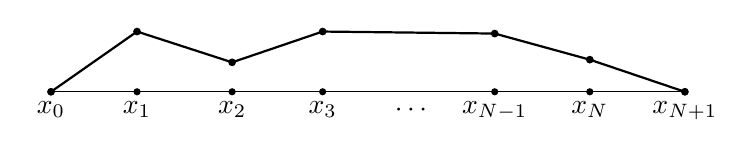
\begin{tikzpicture}[x=1.15cm,y=.85cm]
 \draw[thin] (0,0)--(7,0);
 \draw[thick] (0,0)--(.95,.9)--(2,.44)--(3,.9)--(4.9,.87)--(5.95,.48)--(7,0);
 \foreach \x/\lab/\y in {0/x_0/0,.95/x_1/.9,2/x_2/.44,3/x_3/.9,4.9/x_{N-1}/.87,5.95/x_N/.48,7/x_{N+1}/0}{
   \fill (\x,0) circle (1.3pt) node[below] {$\lab$};
   \fill (\x,\y) circle (1.4pt);
 }
 \node at (4,-.27) {$\cdots$};
\end{tikzpicture}
\end{center}

Each element contributes two local coefficients. Continuity at the \(N\)
interior nodes and the two endpoint conditions impose \(N+2\) independent
constraints. Hence \(\dim V_h=2(N+1)-N-2=N\), the number of interior nodes.
The discrete weak problem is \(a(u_h,v_h)=L(v_h)\) for all \(v_h\in V_h\),
and it gives \(AU=F\) in any basis. A nodal basis satisfies
\(\phi_i(x_j)=\delta_{ij}\) at the interior nodes.

\paragraph{Local interpolation proposition.}
An affine polynomial on \([a_1,a_2]\), \(a_1<a_2\), is determined by its
two endpoint values. If \(p(x)=\beta_0+\beta_1x\) and \(b_i=p(a_i)\),
then
\[
 \begin{pmatrix}1&a_1\\1&a_2\end{pmatrix}
 \begin{pmatrix}\beta_0\\\beta_1\end{pmatrix}
 =\begin{pmatrix}b_1\\b_2\end{pmatrix}.
\]
The determinant is \(a_2-a_1\ne0\). The same polynomial in the Lagrange
basis is
\[
 \begin{gathered}
 p(x)=\ell_1(x)b_1+\ell_2(x)b_2,\qquad \ell_i(a_j)=\delta_{ij},\\
 \ell_1(x)=\frac{x-a_2}{a_1-a_2},\qquad
 \ell_2(x)=\frac{x-a_1}{a_2-a_1}.
 \end{gathered}
\]
Thus \(p\) is the affine graph through \((a_1,b_1)\) and \((a_2,b_2)\).

\begin{center}
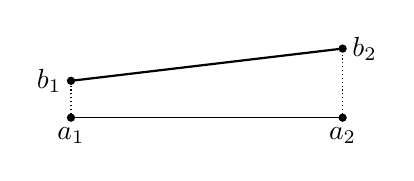
\begin{tikzpicture}[x=1.15cm,y=.65cm]
 \draw (0,0)--(3,0);
 \draw[thick] (0,.72)--(3,1.35);
 \draw[densely dotted] (0,0)--(0,.72) (3,0)--(3,1.35);
 \fill (0,.72) circle (1.5pt) node[left] {$b_1$};
 \fill (3,1.35) circle (1.5pt) node[right] {$b_2$};
 \fill (0,0) circle (1.5pt) node[below] {$a_1$};
 \fill (3,0) circle (1.5pt) node[below] {$a_2$};
\end{tikzpicture}
\end{center}

\clearpage
\section{Lecture 9. Hat functions and matrix assembly}
\lecturesource{Source \enspace\texttt{Lec9\_annotated.pdf}, pp.~1--8}

\subsection{The weak and discrete Dirichlet problems}

On \(I=(0,1)\) consider
\[
 -(a(x)u')'+a_0(x)u=f,\qquad u(0)=u(1)=0,
\]
under the assumptions of Lecture 8. Given \(f\in L^2(I)\), find
\(u\in H_0^1(I)\) such that \(a(u,v)=L(v)\) for all \(v\in H_0^1(I)\), where
\[
 a(u,v)=\int_0^1 a(x)u'v'\,dx+\int_0^1 a_0(x)uv\,dx,\qquad
 L(v)=\int_0^1fv\,dx .
\]
Let \(0=x_0<x_1<\cdots<x_N<x_{N+1}=1\),
\(I_j=[x_{j-1},x_j]\), \(h_j=x_j-x_{j-1}\), and
\(h=\max_{1\le j\le N+1}h_j\). On a uniform mesh, \(h_j=h\) for each \(j\).
Take the conforming linear finite element space
\[
 V_h=\left\{v_h\in C([0,1])\
 \middle|\begin{aligned}
  &v_h|_{I_j}\in P_1(I_j),\quad 1\le j\le N+1\\
  &v_h(0)=v_h(1)=0
 \end{aligned}\right\}\subset H_0^1(I).
\]
The discrete problem is to find \(u_h\in V_h\) satisfying
\[
 a(u_h,v_h)=L(v_h)\qquad(v_h\in V_h).
\]

\paragraph{Exercise.}
Show that the discrete problem is well-posed. Because \(V_h\subset H_0^1(I)\),
the continuous bounds restrict to \(V_h\).
\[
 \begin{aligned}
 a(w_h,w_h)&\ge \alpha\|w_h\|_{H^1(I)}^2,\\
 |a(v_h,w_h)|&\le M\|v_h\|_{H^1(I)}\|w_h\|_{H^1(I)},\\
 |L(v_h)|&\le C\|v_h\|_{H^1(I)} .
 \end{aligned}
\]
Here \(\alpha>0\) follows from \(a(x)\ge\alpha_0>0\), \(a_0(x)\ge0\), and
the Poincar\'e inequality. The coefficient sup norms bound \(M\), and
\(C=\|f\|_{L^2(I)}\) is sufficient. Lax--Milgram gives a unique \(u_h\) and
\(\|u_h\|_{H^1(I)}\le C/\alpha\).

\subsection{Construction of the nodal basis}

On an element \([a_1,a_2]\), a linear polynomial \(p(x)=c_1+c_2x\) has
the representation \(p(x)=\ell_1(x)b_1+\ell_2(x)b_2\),
where \(b_j=p(a_j)\) and
\[
 \ell_1(x)=\frac{a_2-x}{a_2-a_1},\qquad
 \ell_2(x)=\frac{x-a_1}{a_2-a_1},\qquad
 \ell_i(a_j)=\delta_{ij}.
\]
The Kronecker delta is \(1\) when \(i=j\) and \(0\) otherwise.
\begin{center}
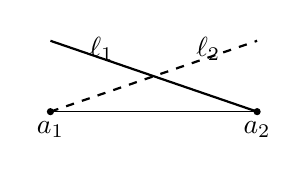
\begin{tikzpicture}[x=1.05cm,y=.9cm]
 \draw (0,0)--(2.5,0);
 \draw[thick] (0,1)--(2.5,0);
 \draw[thick,dashed] (0,0)--(2.5,1);
 \node at (.62,.88) {$\ell_1$};
 \node at (1.91,.89) {$\ell_2$};
 \fill (0,0) circle (1.3pt) node[below] {$a_1$};
 \fill (2.5,0) circle (1.3pt) node[below] {$a_2$};
\end{tikzpicture}
\end{center}

Construct global basis functions with \(\phi_i(x_j)=\delta_{ij}\) at
the interior nodes \(1\le i,j\le N\). For each \(i\), the \emph{hat function}
\(\phi_i\) is
\[
 \phi_i(x)=
 \begin{cases}
 (x-x_{i-1})/h_i, & x_{i-1}\le x\le x_i,\\[2pt]
 (x_{i+1}-x)/h_{i+1}, & x_i<x\le x_{i+1},\\
 0, & \text{otherwise}.
 \end{cases}
 \qquad \operatorname{supp}\phi_i=[x_{i-1},x_{i+1}].
\]
\begin{center}
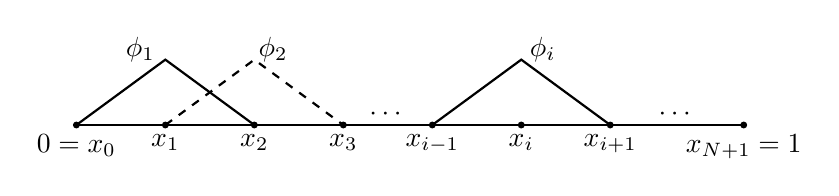
\begin{tikzpicture}[x=1.13cm,y=.83cm]
 \draw (0,0)--(7.5,0);
 \draw[thick] (0,0)--(1,1)--(2,0);
 \draw[thick,dashed] (1,0)--(2,1)--(3,0);
 \draw[thick] (4,0)--(5,1)--(6,0);
 \node at (.72,1.16) {$\phi_1$};
 \node at (2.21,1.16) {$\phi_2$};
 \node at (5.24,1.16) {$\phi_i$};
 \foreach \x/\lab in {0/0=x_0,1/x_1,2/x_2,3/x_3,4/x_{i-1},5/x_i,6/x_{i+1},7.5/x_{N+1}=1}
  \fill (\x,0) circle (1.25pt) node[below] {$\lab$};
 \node at (3.5,.16) {$\cdots$};
 \node at (6.75,.16) {$\cdots$};
\end{tikzpicture}
\end{center}

These \(N\) hats belong to \(V_h\). Evaluating a linear combination at
\(x_j\) recovers its \(j\)-th coefficient, so the hats are linearly
independent and form a basis of the \(N\)-dimensional space.
For \(u_h=\sum_{i=1}^N\alpha_i\phi_i\),
\[
 u_h(x_j)=\sum_{i=1}^N\alpha_i\phi_i(x_j)=\alpha_j,
 \qquad
 u_h(x)=\sum_{i=1}^N u_h(x_i)\phi_i(x).
\]
For example, on the mesh \(0=x_0<x_1<x_2<x_3=1\), if
\(v_h(x_1)=0.1\) and \(v_h(x_2)=0.7\), then
\(v_h=0.1\phi_1+0.7\phi_2\). Its graph joins the two endpoint values
\(0\) through these two interior nodal values.

\subsection{Matrix entries, sparsity, and positive definiteness}

Testing with \(\phi_j\) gives \(AU=F\) with
\[
 A_{ji}=a(\phi_i,\phi_j),\qquad U=(\alpha_i)_{i=1}^N,\qquad
 F=(L(\phi_j))_{j=1}^N.
\]
Let \(i,j\) label hats and \(k\) label mesh elements. Splitting the two
integrals gives
\[
 a(\phi_i,\phi_j)
 =\sum_{k=1}^{N+1}\left(
   \int_{I_k}a(x)\phi_i'\phi_j'\,dx+
   \int_{I_k}a_0(x)\phi_i\phi_j\,dx
 \right).
\]
For fixed \(i\), a nonzero entry can occur only for \(j=i-1,i,i+1\)
within \(1,\ldots,N\). Supports beyond those neighbors are disjoint
except possibly for a mesh point, which contributes zero to a volume
integral. Thus \(A\) is tridiagonal.

For \(\mathbf v=(v_1,\ldots,v_N)^{\mathsf T}\) let
\(v_h=\sum_{i=1}^Nv_i\phi_i\). Bilinearity and coercivity give
\[
 \mathbf v^{\mathsf T}A\mathbf v
 =\sum_{i,j=1}^N a(\phi_i,\phi_j)v_iv_j
 =a(v_h,v_h)\ge\alpha\|v_h\|_{H^1(I)}^2 .
\]
Independence of the hats gives \(v_h\ne0\) for \(\mathbf v\ne0\).
The bilinear form is symmetric, so \(A\) is symmetric positive definite.

\subsection{Uniform-mesh assembly for unit coefficients}

Let \(a(x)=a_0(x)=1\) and \(h=1/(N+1)\). Split the form into the
gradient part \(b\) and the mass part \(c\).
\[
 a(\phi_i,\phi_j)=b(\phi_i,\phi_j)+c(\phi_i,\phi_j),\qquad
 \begin{aligned}
 b(\phi_i,\phi_j)&=\sum_{k=1}^{N+1}\int_{I_k}\phi_i'\phi_j'\,dx,\\
 c(\phi_i,\phi_j)&=\sum_{k=1}^{N+1}\int_{I_k}\phi_i\phi_j\,dx.
 \end{aligned}
\]
For the three hats \(s=i-1,i,i+1\) that meet \(\phi_i\), use the
formula from the preceding subsection with index \(s\). Their positive
and negative slopes lie on the following intervals, with derivative
zero outside the two listed intervals.
\[
 \begin{array}{c|cc}
 \text{hat} & +1/h & -1/h\\ \hline
 \phi_{i-1} &(x_{i-2},x_{i-1})&(x_{i-1},x_i)\\
 \phi_i &(x_{i-1},x_i)&(x_i,x_{i+1})\\
 \phi_{i+1} &(x_i,x_{i+1})&(x_{i+1},x_{i+2})
 \end{array}
\]
Use each row only when its hat index lies in \(\{1,\ldots,N\}\).
For these indices,
\[
\begin{aligned}
 b(\phi_i,\phi_{i-1})
 &=\int_{x_{i-1}}^{x_i}\phi_i'\phi_{i-1}'\,dx
   =h(1/h)(-1/h)=-1/h,\\
 b(\phi_i,\phi_i)
 &=\int_{x_{i-1}}^{x_i}(\phi_i')^2\,dx+
   \int_{x_i}^{x_{i+1}}(\phi_i')^2\,dx
   =2/h,\\
 b(\phi_i,\phi_{i+1})
 &=\int_{x_i}^{x_{i+1}}\phi_i'\phi_{i+1}'\,dx
   =h(-1/h)(1/h)=-1/h.
\end{aligned}
\]
Thus the gradient matrix is
\(B=h^{-1}\operatorname{tridiag}(-1,2,-1)\), where
\(\operatorname{tridiag}(l,d,r)\) has subdiagonal \(l\), diagonal \(d\),
and superdiagonal \(r\).

For the mass contribution, the overlap integrals are
\[
\begin{aligned}
 c(\phi_i,\phi_{i-1})&=\int_{x_{i-1}}^{x_i}\phi_i\phi_{i-1}\,dx,\\
 c(\phi_i,\phi_i)&=\int_{x_{i-1}}^{x_i}\phi_i^2\,dx+
                     \int_{x_i}^{x_{i+1}}\phi_i^2\,dx,\\
 c(\phi_i,\phi_{i+1})&=\int_{x_i}^{x_{i+1}}\phi_i\phi_{i+1}\,dx .
\end{aligned}
\]
On an element \([a,b]\), Simpson's \(1/3\) rule is
\[
 \int_a^b g(x)\,dx\ \approx\
 \frac{b-a}{6}\left(g(a)+4g\bigl((a+b)/2\bigr)+g(b)\right).
\]
The products here are quadratic on the element, so the rule integrates
them exactly. Two adjacent hats take the endpoint pairs \((0,1)\)
and \((1,0)\), and their product takes values \(0,1/4,0\) at the left,
midpoint, and right. This gives \(h/6\). Squaring one hat on one
of its elements gives endpoint values \(0,1\) or \(1,0\) and midpoint
value \(1/4\). This gives \(h/3\) per element and \(2h/3\) on its
two-element support. Therefore \(C=(h/6)\operatorname{tridiag}(1,4,1)\)
and \(A=B+C\).

The load uses the same support restriction.
\[
 F_j=L(\phi_j)
 =\sum_{k=1}^{N+1}\int_{I_k}f\phi_j\,dx
 =\int_{x_{j-1}}^{x_j}f\phi_j\,dx+
   \int_{x_j}^{x_{j+1}}f\phi_j\,dx .
\]
Use element quadrature to evaluate these two integrals when \(f\) is
available at quadrature points. The assembled system determines
\[
 U=A^{-1}F=(u_h(x_1),\ldots,u_h(x_N))^{\mathsf T}.
\]
\emph{Index correction.} Element sums run over \(1,\ldots,N+1\).
the Dirichlet matrix and load use the \(N\) interior hats.

\clearpage
\section{Lecture 10. Quadratic elements and Neumann data}
\lecturesource{Source \enspace\texttt{Lec10\_annotated.pdf}, pp.~1--7}

\subsection{Linear conforming elements for the Dirichlet problem}

Let \(\Omega=(0,1)\) and consider
\[
 -u''+u=f\quad\text{in }(0,1),\qquad
 u(0)=u(1)=0,\qquad f\in L^2(0,1).
\]
Find \(u\in H_0^1(0,1)\) satisfying \(a(u,v)=L(v)\) for all
\(v\in H_0^1(0,1)\), with
\[
 a(u,v)=\int_0^1u'v'\,dx+\int_0^1uv\,dx,\qquad L(v)=\int_0^1fv\,dx.
\]
Write \(I_j=[x_{j-1},x_j]\), \(j=1,\ldots,N+1\), for the mesh of
\(0=x_0<\cdots<x_N<x_{N+1}=1\). In the linear finite element approximation,
\[
 V_h=\bigl\{v_h\in C([0,1]):v_h|_{I_j}\in P_1(I_j)
 \text{ for }1\le j\le N+1,\ v_h(0)=v_h(1)=0\bigr\}.
\]
The inclusion \(V_h\subset H_0^1(0,1)\) makes the method conforming.
A discrete space outside the trial space leads to a nonconforming
method. For example, discontinuous Galerkin uses functions that may
jump at element interfaces.

The \(N\) interior hats \(\phi_i\) form a basis. For
\(u_h=\sum_{i=1}^N\alpha_i\phi_i\), the discrete weak equation
\(a(u_h,v_h)=L(v_h)\) for all \(v_h\in V_h\) gives \(AU=F\), with
\(A_{ji}=a(\phi_i,\phi_j)\), \(U=(\alpha_i)_{i=1}^N\), and
\(F=(L(\phi_j))_{j=1}^N\).

The questions in the lecture concern convergence as \(h\to0\) in the
\(H^1\) and \(L^2\) norms. For this one-dimensional equation,
\(u\in H^2(0,1)\), since \(u''=u-f\in L^2(0,1)\).
The linear conforming method satisfies
\[
 \|u-u_h\|_{H^1(0,1)}=O(h),\qquad
 \|u-u_h\|_{L^2(0,1)}=O(h^2).
\]
\emph{Derivation of the stated rates.} Galerkin orthogonality and the piecewise-linear interpolation estimate give
the \(H^1\) bound. Indeed, for the nodal interpolant \(I_hu\),
\(\|u-u_h\|_{H^1}\le\|u-I_hu\|_{H^1}\le Ch\|u\|_{H^2}\),
since \(a\) is the \(H^1\) inner product. For \(e=u-u_h\), solve
\(-z''+z=e\) with homogeneous Dirichlet data. Then
\(\|z\|_{H^2}\le C\|e\|_{L^2}\) and
\[
 \|e\|_{L^2}^2=a(e,z)=a(e,z-I_hz)
 \le Ch\|e\|_{H^1}\|e\|_{L^2},
\]
which yields the \(L^2\) rate.

\subsection{Quadratic conforming finite element space}

Keep the mesh and replace \(P_1(I_j)\) on each element by \(P_2(I_j)\).
\[
 V_h=\bigl\{v_h\in C([0,1]):v_h|_{I_j}\in P_2(I_j)
 \text{ for }1\le j\le N+1,\ v_h(0)=v_h(1)=0\bigr\}.
\]
\emph{Check.} Show \(V_h\subset H_0^1(0,1)\). The elementwise derivative
is piecewise linear and lies in \(L^2(0,1)\). Continuity cancels the
interior endpoint terms from integration by parts, giving the weak
derivative. The endpoint values are zero.

\emph{Exercise.} Prove well-posedness of the discrete problem
\(a(u_h,v_h)=L(v_h)\) for all \(v_h\in V_h\). The continuous
coercivity and boundedness estimates restrict to the subspace \(V_h\),
so Lax--Milgram applies.

Let \(N_d=\dim V_h\) and choose a basis
\(\{\psi_1,\ldots,\psi_{N_d}\}\). Writing \(u_h\) in this basis, we have
\[
 \begin{gathered}
 a\Bigl(\sum_{i=1}^{N_d}\alpha_i\psi_i,v_h\Bigr)=L(v_h)
 \quad(v_h\in V_h)\\
 \Updownarrow\\
 \sum_{i=1}^{N_d}\alpha_i a(\psi_i,\psi_j)=L(\psi_j)
 \quad(1\le j\le N_d).
 \end{gathered}
\]
This is \(AU=F\) with \(A_{ji}=a(\psi_i,\psi_j)\),
\(U=(\alpha_i)_{i=1}^{N_d}\), and \(F=(L(\psi_j))_{j=1}^{N_d}\).

\subsection{Local quadratic interpolation}

\paragraph{Proposition.}
A polynomial \(p\in P_2([a_1,a_2])\), with \(a_1<a_2\), is uniquely
determined by its values at \(a_1,a_2\) and the midpoint
\(a_3=(a_1+a_2)/2\). If \(p(x)=c_0+c_1x+c_2x^2\) and \(b_i=p(a_i)\),
the coefficients solve
\[
 \begin{pmatrix}1&a_1&a_1^2\\1&a_2&a_2^2\\1&a_3&a_3^2\end{pmatrix}
 \begin{pmatrix}c_0\\c_1\\c_2\end{pmatrix}
 =\begin{pmatrix}b_1\\b_2\\b_3\end{pmatrix}.
\]
A polynomial of degree at most two with three distinct roots is zero,
so the homogeneous system has only the zero solution. The local
Lagrange basis is
\[
\begin{aligned}
 \ell_1(x)&=\frac{(x-a_2)(x-a_3)}{(a_1-a_2)(a_1-a_3)},&
 \ell_2(x)&=\frac{(x-a_1)(x-a_3)}{(a_2-a_1)(a_2-a_3)},\\
 \ell_3(x)&=\frac{(x-a_1)(x-a_2)}{(a_3-a_1)(a_3-a_2)}.&
\end{aligned}
\]
These satisfy \(\ell_i(a_j)=\delta_{ij}\) and
\(p(x)=\sum_{i=1}^{3}\ell_i(x)b_i\).

\begin{center}
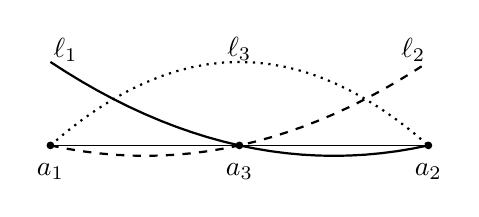
\begin{tikzpicture}[x=1.6cm,y=1.06cm]
 \draw (0,0)--(3,0);
 \begin{scope}[xscale=3]
  \draw[thick] plot[domain=0:1,samples=25] (\x,{2*(\x-1)*(\x-.5)});
  \draw[thick,dashed] plot[domain=0:1,samples=25] (\x,{2*\x*(\x-.5)});
  \draw[thick,dotted] plot[domain=0:1,samples=25] (\x,{4*\x*(1-\x)});
 \end{scope}
 \node at (.12,1.14) {$\ell_1$};
 \node at (2.88,1.14) {$\ell_2$};
 \node at (1.5,1.16) {$\ell_3$};
 \fill (0,0) circle (1.4pt) node[below=3pt] {$a_1$};
 \fill (1.5,0) circle (1.4pt) node[below=3pt] {$a_3$};
 \fill (3,0) circle (1.4pt) node[below=3pt] {$a_2$};
\end{tikzpicture}
\end{center}

\subsection{Global quadratic nodal basis}

Let \(m_j=(x_{j-1}+x_j)/2\) for \(1\le j\le N+1\). Each element
has three polynomial coefficients. Continuity at the \(N\) interior
vertices and the two endpoint conditions give
\[
  N_d=\dim V_h=3(N+1)-N-2=2N+1=N+(N+1).
\]
The degrees of freedom are the \(N\) interior vertex values and the
\(N+1\) element midpoint values. Local quadratic interpolation on adjacent
elements uses the same value at their shared vertex, so these degrees of
freedom determine a unique global member of \(V_h\).

\begin{center}
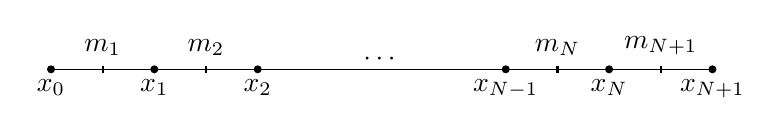
\begin{tikzpicture}[x=1.05cm,y=.86cm]
 \draw (0,0)--(8,0);
 \foreach \x/\lab in {0/x_0,1.25/x_1,2.5/x_2,5.5/x_{N-1},6.75/x_N,8/x_{N+1}}
   \fill (\x,0) circle (1.45pt) node[below] {$\lab$};
 \foreach \x/\lab in {.625/m_1,1.875/m_2,6.125/m_N,7.375/m_{N+1}}
   \draw[thick] (\x,-.055)--(\x,.055) node[above] {$\lab$};
 \node at (4,.15) {$\cdots$};
\end{tikzpicture}
\end{center}

Let \(\phi_{x_i}\) be the vertex function and \(\phi_{m_i}\) the
midpoint function. Their nodal values are
\[
\begin{aligned}
 \phi_{x_i}(x_j)&=\delta_{ij} &&(1\le i,j\le N),\\
 \phi_{x_i}(m_j)&=0 &&(1\le i\le N,\ 1\le j\le N+1),\\
 \phi_{m_i}(m_j)&=\delta_{ij} &&(1\le i,j\le N+1),\\
 \phi_{m_i}(x_j)&=0 &&(1\le i\le N+1,\ 0\le j\le N+1).
\end{aligned}
\]
All vertex functions vanish at \(x_0,x_{N+1}\). For \(1\le i\le N\) the
local Lagrange formulas give
\[
 \phi_{x_i}(x)=
 \begin{cases}
 \dfrac{(x-x_{i-1})(x-m_i)}{(x_i-x_{i-1})(x_i-m_i)},
    & x\in[x_{i-1},x_i],\\[6pt]
 \dfrac{(x-x_{i+1})(x-m_{i+1})}{(x_i-x_{i+1})(x_i-m_{i+1})},
    & x\in(x_i,x_{i+1}],\\[6pt]
 0,&\text{otherwise}.
 \end{cases}
\]
For \(1\le i\le N+1\),
\[
 \phi_{m_i}(x)=
 \begin{cases}
 \dfrac{(x-x_{i-1})(x-x_i)}{(m_i-x_{i-1})(m_i-x_i)},
      &x\in[x_{i-1},x_i],\\[6pt]
 0,&\text{otherwise}.
 \end{cases}
\]
Thus \(\operatorname{supp}\phi_{x_i}=[x_{i-1},x_{i+1}]\) and
\(\operatorname{supp}\phi_{m_i}=[x_{i-1},x_i]\).

\begin{center}
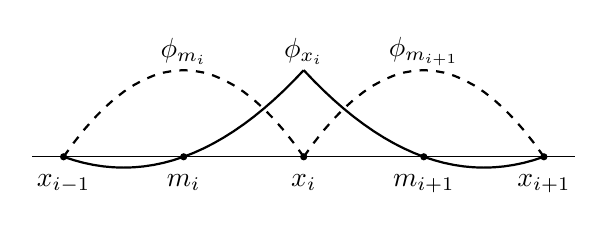
\begin{tikzpicture}[x=3.05cm,y=1.1cm]
 \draw (-.13,0)--(2.13,0);
 \draw[thick] plot[domain=0:1,samples=25] (\x,{2*\x*(\x-.5)});
 \draw[thick] plot[domain=1:2,samples=25] (\x,{2*(\x-2)*(\x-1.5)});
 \draw[thick,dashed] plot[domain=0:1,samples=25] (\x,{4*\x*(1-\x)});
 \draw[thick,dashed] plot[domain=1:2,samples=25] (\x,{4*(\x-1)*(2-\x)});
 \node at (.5,1.22) {$\phi_{m_i}$};
 \node at (1,1.22) {$\phi_{x_i}$};
 \node at (1.5,1.22) {$\phi_{m_{i+1}}$};
 \foreach \x/\lab in {0/x_{i-1},.5/m_i,1/x_i,1.5/m_{i+1},2/x_{i+1}}
  \fill (\x,0) circle (1.3pt) node[below=3pt] {$\lab$};
\end{tikzpicture}
\end{center}

In the global ordering, the midpoint \(m_j\) has degree-of-freedom
index \(N+j\). Thus
\[
 \psi_i=
 \begin{cases}
 \phi_{x_i},&1\le i\le N,\\
 \phi_{m_{i-N}},&N+1\le i\le2N+1 .
 \end{cases}
\]
The coefficient of a basis function equals the discrete solution at its
node. In fact, for \(1\le j\le N\),
\[
 u_h(x_j)=\sum_{i=1}^N\alpha_i\phi_{x_i}(x_j)
       +\sum_{i=1}^{N+1}\alpha_{N+i}\phi_{m_i}(x_j)=\alpha_j.
\]
For \(1\le j\le N+1\), the vertex terms vanish at \(m_j\), and
\[
 u_h(m_j)=\sum_{i=1}^N\alpha_i\phi_{x_i}(m_j)
       +\sum_{i=1}^{N+1}\alpha_{N+i}\phi_{m_i}(m_j)=\alpha_{N+j}.
\]
Consequently,
\[
 U=\bigl(u_h(x_1),\ldots,u_h(x_N),u_h(m_1),\ldots,u_h(m_{N+1})\bigr)^{\mathsf T}.
\]
\emph{Index correction.} The handwritten final midpoint coefficient
mixes local midpoint indices and global basis indices. The coefficient
for \(m_j\) is \(\alpha_{N+j}\).

Assemble the matrix from integrals on \(I_k\), \(1\le k\le N+1\).
The lecture suggests Gauss quadrature for terms such as
\(\int_{I_k}\psi_i\psi_j\,dx\). With unit coefficients, the product of
two quadratic shape functions has degree at most four on each element,
so a three-point Gauss rule is exact. The product of two elementwise
derivatives has degree at most two, so a two-point Gauss rule is exact.

\pagebreak[4]
\subsection{Linear conforming elements for the Neumann problem}

Consider
\[
 -u''+u=f\quad\text{in }(0,1),\qquad u'(0)=u'(1)=0.
\]
Find \(u\in H^1(0,1)\) such that
\[
 \int_0^1u'v'\,dx+\int_0^1uv\,dx=\int_0^1fv\,dx
 \qquad(v\in H^1(0,1)).
\]
The boundary term vanishes because the endpoint fluxes are zero.
The reaction term gives coercivity on \(H^1(0,1)\). The linear
conforming space is
\[
 V_h=\bigl\{v_h\in C([0,1]):v_h|_{I_j}\in P_1(I_j)
       \text{ for }1\le j\le N+1\bigr\}\subset H^1(0,1).
\]
Its dimension is \(2(N+1)-N=N+2\), the number of vertices, because
continuity gives \(N\) constraints and endpoint values are free.
Keep the usual interior hats and add the two endpoint functions.
\[
 \begin{aligned}
 \phi_0(x)=
 \begin{cases}
 \dfrac{x-x_1}{x_0-x_1},&x\in[x_0,x_1],\\[4pt]
 0,&\text{otherwise},
 \end{cases}\\[4pt]
 \phi_{N+1}(x)=
 \begin{cases}
 \dfrac{x-x_N}{x_{N+1}-x_N},&x\in[x_N,x_{N+1}],\\[4pt]
 0,&\text{otherwise}.
 \end{cases}
 \end{aligned}
\]
For example, \(\phi_0(x_0)=1\) and \(\phi_0(x_j)=0\) for \(j>0\).

\begin{center}
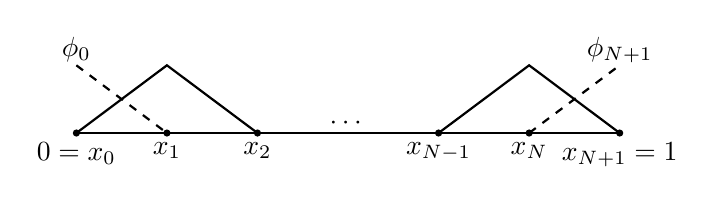
\begin{tikzpicture}[x=1.15cm,y=.86cm]
 \draw (0,0)--(6,0);
 \draw[thick] (0,0)--(1,1)--(2,0) (4,0)--(5,1)--(6,0);
 \draw[thick,dashed] (0,1)--(1,0) (5,0)--(6,1);
 \node at (0,1.23) {$\phi_0$};
 \node at (6,1.23) {$\phi_{N+1}$};
 \foreach \x/\lab in {0/0=x_0,1/x_1,2/x_2,4/x_{N-1},5/x_N,6/x_{N+1}=1}
   \fill (\x,0) circle (1.3pt) node[below] {$\lab$};
 \node at (3,.14) {$\cdots$};
\end{tikzpicture}
\end{center}

The full basis \(\{\phi_i\}_{i=0}^{N+1}\) satisfies
\(\phi_i(x_j)=\delta_{ij}\). Expand
\(u_h=\sum_{i=0}^{N+1}\alpha_i\phi_i\) with \(\alpha_i=u_h(x_i)\).
The Galerkin system is
\[
 \begin{gathered}
 AU=F,\qquad A_{ji}=a(\phi_i,\phi_j),\qquad 0\le i,j\le N+1,\\
 U=(\alpha_i)_{i=0}^{N+1},\qquad F=(L(\phi_j))_{j=0}^{N+1}.
 \end{gathered}
\]

\clearpage
\section{Lecture 11. Conforming finite elements in two dimensions}
\lecturesource{Source \enspace\texttt{Lec11\_annotated.pdf}, pp.~1--9}

\subsection{From the 1D problem to a polygonal domain}

On \(I=(0,1)\) the model problem is \(-u''+u=f\) with \(u(0)=u(1)=0\).
Its weak formulation is to find \(u\in H_0^1(I)\) such that
\[
 a(u,v)=L(v)\quad(v\in H_0^1(I)),\qquad
 a(u,v)=\int_I (u'v'+uv)\,dx,\qquad L(v)=\int_I fv\,dx.
\]
On a partition into intervals \(I_j\), choose the continuous piecewise
polynomials of degree at most \(k\), for an integer \(k\geq 1\), that vanish
at the endpoints. This is a conforming subspace \(V_h\subset H_0^1(I)\).
The finite element approximation satisfies \(a(u_h,v_h)=L(v_h)\) for all
\(v_h\in V_h\).

Now let \(\Omega\subset\mathbb R^2\) be an open, bounded polygonal domain.
The unit square and an L-shaped domain are examples. The abstract weak
problem on a Hilbert space \(V\) is to find \(u\in V\) such that
\(a(u,v)=L(v)\) for all \(v\in V\). The two model boundary conditions for
\(-\Delta u+u=f\) are
\[
\begin{array}{ccl}
\text{Dirichlet} & u=0\ \text{on }\partial\Omega & V=H_0^1(\Omega),\\
\text{Neumann} & \partial_n u=0\ \text{on }\partial\Omega & V=H^1(\Omega).
\end{array}
\]
Both use
\[
 a(u,v)=\int_\Omega \bigl(\nabla u\cdot\nabla v+uv\bigr)\,dx,
 \qquad L(v)=\int_\Omega fv\,dx.
\]
A conforming discretization uses a mesh of \(\overline\Omega\), a
finite-dimensional subspace \(V_h\subset V\), and the discrete weak problem
on \(V_h\).

\subsection{Mesh, element polynomials, and support}

A triangulation \(\mathcal T_h=\{T_1,\ldots,T_{N_E}\}\) subdivides
\(\overline\Omega\) into closed elements. The lecture includes rectangular
meshes as a second example of a subdivision. For the triangular mesh, the
conditions are
\begin{enumerate}
\item \(\bigcup_{j=1}^{N_E}T_j=\overline\Omega\).
\item Distinct elements have disjoint interiors.
\item Each element boundary is Lipschitz.
\item Two distinct elements intersect in the empty set, a common vertex,
or a common edge.
\end{enumerate}

\begin{center}
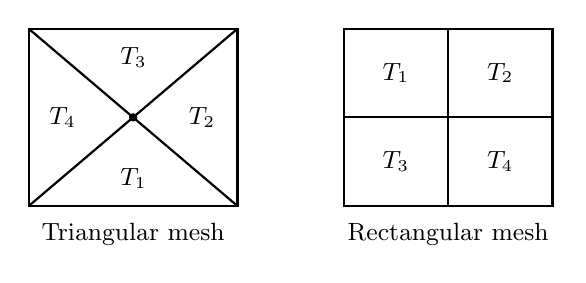
\begin{tikzpicture}[x=1.0cm,y=1.0cm,thick,every node/.style={font=\small}]
\draw (0,0) rectangle (2.65,2.25);
\draw (0,0)--(2.65,2.25) (0,2.25)--(2.65,0);
\node at (1.33,0.35) {\(T_1\)};
\node at (2.2,1.12) {\(T_2\)};
\node at (1.33,1.89) {\(T_3\)};
\node at (0.43,1.12) {\(T_4\)};
\fill (1.325,1.125) circle (1.5pt);
\node[below] at (1.325,-0.09) {Triangular mesh};
\begin{scope}[xshift=4.0cm]
\draw (0,0) rectangle (2.65,2.25);
\draw (0,1.125)--(2.65,1.125) (1.325,0)--(1.325,2.25);
\node at (0.6625,1.6875) {\(T_1\)};
\node at (1.9875,1.6875) {\(T_2\)};
\node at (0.6625,0.5625) {\(T_3\)};
\node at (1.9875,0.5625) {\(T_4\)};
\node[below] at (1.325,-0.09) {Rectangular mesh};
\end{scope}
\end{tikzpicture}
\end{center}

The functions in \(V_h\) are piecewise polynomial. The restrictions
\(\{v_h|_T:v_h\in V_h\}\) form a local polynomial space on \(T\).
A finite element basis is chosen with small supports, so each basis
function is zero on most of the mesh. For example, \(P_k(T)\) is the space
of restrictions to \(T\) of polynomials of total degree at most \(k\).
Using multi-index notation in \(\mathbb R^n\),
\[
 p(x)=\sum_{|\alpha|\leq k} c_\alpha x^\alpha,\qquad
 x^\alpha=x_1^{\alpha_1}\cdots x_n^{\alpha_n},\qquad
 |\alpha|=\alpha_1+\cdots+\alpha_n .
\]

\subsection{Why continuous piecewise polynomials belong to \(H^1\)}

Let \(v_h\in C(\overline\Omega)\) be polynomial on every element.
Then \(v_h\in H^1(\Omega)\), and its weak derivatives equal its
elementwise derivatives almost everywhere.

To prove the claim, define \(w_i\in L^2(\Omega)\) by
\(w_i|_T=\partial_i(v_h|_T)\), for \(i=1,2\). For a test function
\(\varphi\in C_c^\infty(\Omega)\), integrate by parts on each element.
\[
 \int_T w_i\varphi\,dx
 =-\int_T v_h\,\partial_i\varphi\,dx
   +\int_{\partial T}(v_h|_T)\varphi\,n_{i,T}\,ds,
\]
where \(n_{i,T}\) is the \(i\)-th component of the outward unit normal.
Write \(\mathcal E_h=\mathcal E_h^{\mathrm{int}}\cup\mathcal E_h^\partial\)
for the interior and boundary edges. The sum of the boundary integrals
over \(T\in\mathcal T_h\) takes the following form.
\[
 \sum_{e\in\mathcal E_h^{\mathrm{int}}}
 \int_e \bigl(v_h|_{T^+}-v_h|_{T^-}\bigr)\varphi\,n_{i,T^+}\,ds
 +\sum_{e\in\mathcal E_h^\partial}
 \int_e v_h\,\varphi\,n_{i,T}\,ds .
\]
On an interior edge the adjacent normals have opposite signs and the
two traces of \(v_h\) coincide. On a boundary edge \(\varphi=0\).
Summing therefore gives
\[
 \int_\Omega w_i\varphi\,dx=-\int_\Omega v_h\,\partial_i\varphi\,dx.
\]
Thus \(w_i=\partial_i v_h\) in the weak sense. If \(v_h=0\) on
\(\partial\Omega\), its trace vanishes and \(v_h\in H_0^1(\Omega)\).

\textbf{Exercise.} Prove the same statement in one dimension by summing
integration by parts over the mesh intervals. At every interior node,
the two endpoint terms cancel.

\textbf{Remark.} If a piecewise-polynomial \(v_h\) is \(C^1\) across
the mesh, the same argument applies to its first derivatives, giving
\(v_h\in H^2(\Omega)\). This extra regularity is relevant to the clamped
biharmonic problem
\[
 \Delta^2u=f\ \text{in }\Omega,\qquad
 u=0,\quad \partial_nu=0\ \text{on }\partial\Omega.
\]

\subsection{Discrete Dirichlet problem and its matrix form}

For the homogeneous Dirichlet problem on a triangular mesh use
\[
 V_h=\bigl\{v_h\in C(\overline\Omega):
 v_h|_T\in P_k(T)\ \text{for every }T\in\mathcal T_h,\quad
 v_h=0\text{ on }\partial\Omega\bigr\}\subset H_0^1(\Omega).
\]
Find \(u_h\in V_h\) such that \(a(u_h,v_h)=L(v_h)\) for all \(v_h\in V_h\).

\textbf{Exercise.} Show that this discrete problem is well posed. The
continuity and coercivity of \(a\) and the boundedness of \(L\) carry over
from \(V\) to \(V_h\). For the model problem
\(a(v_h,v_h)=\|v_h\|_{H^1(\Omega)}^2\).

Let \(N_d=\dim V_h\) and choose a basis \(\{\phi_1,\ldots,\phi_{N_d}\}\).
Writing \(u_h=\sum_{i=1}^{N_d}\alpha_i\phi_i\) and testing with each
\(\phi_j\) gives
\[
 \sum_{i=1}^{N_d} a(\phi_i,\phi_j)\alpha_i=L(\phi_j),
 \qquad 1\leq j\leq N_d .
\]
Hence \(AU=F\) where \(U=(\alpha_i)_i\), \(F_j=L(\phi_j)\), and the
row-\(j\), column-\(i\) entry is \(A_{ji}=a(\phi_i,\phi_j)\).
For this symmetric bilinear form \(A_{ji}=a(\phi_j,\phi_i)\) as well.

\clearpage
\section{Lecture 12. Vertex degrees of freedom on triangles}

\editorialnote{\textbf{Reconstructed lecture.} Lecture 11 ends with an
abstract basis for the 2D Galerkin system. Lecture 13, p.~1, recalls two
\(P_1\) spaces, the interior and boundary vertex sets, and the corresponding
dimension counts. The proof below reconstructs that transition.}

\subsection{Vertex values determine the global function}

Let \(\mathcal T_h\) be a triangulation of \(\overline\Omega\).
Write \(\mathcal V_h=\mathcal V_h^i\cup\mathcal V_h^b\) for all mesh vertices,
with \(\mathcal V_h^i\) the interior vertices and \(\mathcal V_h^b\) the
vertices on \(\partial\Omega\). Set
\[
 \begin{aligned}
  \overline V_h
    &=\{v_h\in C(\overline\Omega):
        v_h|_T\in P_1(T)\text{ for every }T\in\mathcal T_h\},\\
  V_h
    &=\{v_h\in \overline V_h:v_h(a)=0
        \text{ for every }a\in\mathcal V_h^b\}.
 \end{aligned}
\]
A polynomial in \(P_1(T)\) has the form \(c_0+c_1x_1+c_2x_2\).
The three vertices of a nondegenerate triangle are noncollinear, so
prescribing the value at each vertex yields three independent equations
for the three coefficients. Equivalently, an affine function that is
zero at all three vertices is zero on \(T\).

Assign a value to each global mesh vertex. The local affine interpolants
on two neighboring triangles agree at both endpoints of their shared edge.
Their restrictions to that edge are affine in one variable and hence
agree along the entire edge. This makes the interpolants a continuous
global function. The correspondence between a function in \(\overline V_h\)
and its vertex values is therefore a linear isomorphism. In particular,
\[
 \dim\overline V_h=\#\mathcal V_h.
\]

A linear function with zero values at both ends of a boundary edge
vanishes along that edge. The Dirichlet condition leaves one free value per interior vertex.
The conformity argument from Lecture 11 then gives
\[
 \overline V_h\subset H^1(\Omega),\qquad
 V_h\subset H_0^1(\Omega),\qquad
 \dim V_h=\#\mathcal V_h^i.
\]

\subsection{A mesh with one free vertex}

Split a square into four triangles by joining its center to the corners.
The corner values determine four of the vertex degrees of freedom.
With zero Dirichlet values at the corners, the center value determines
the whole function.

\begin{center}
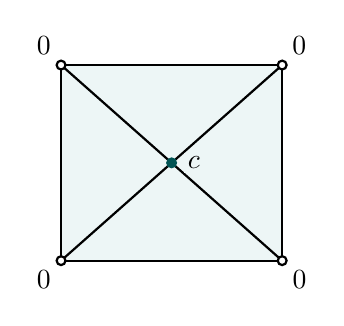
\begin{tikzpicture}[x=1.08cm,y=1.08cm,thick]
\draw[fill=teal!7] (0,0) rectangle (2.6,2.3);
\draw (0,0)--(2.6,2.3) (0,2.3)--(2.6,0);
\foreach \x/\y/\s in {0/0/below left,2.6/0/below right,2.6/2.3/above right,0/2.3/above left}{
  \filldraw[fill=white] (\x,\y) circle (1.6pt) node[\s] {\(0\)};
}
\fill[teal!65!black] (1.3,1.15) circle (2pt);
\node[fill=teal!7,inner sep=1.5pt,right=4pt] at (1.3,1.15) {\(c\)};
\end{tikzpicture}
\end{center}

Taking \(c=1\) gives the nodal hat function for the center. On a general
mesh, prescribe one at an interior vertex and zero at every other
vertex to obtain its hat function. The piecewise affine construction
shows that the function vanishes on triangles that do not contain its
vertex. The explicit local formulas are developed in Lecture 13.

\clearpage
\section{Lecture 13. Simplices, barycentric coordinates, and the nodal basis}
\lecturesource{Source \enspace\texttt{Lec13\_annotated.pdf}, pp.~1--9}

\subsection{Recall of the linear finite element spaces}

Let \(\Omega\subset\mathbb R^2\) be open, bounded, and polygonal, and
let \(\mathcal T_h\) be a triangulation. The continuous, piecewise affine
space \(\overline V_h\subset H^1(\Omega)\) has dimension \(\#\mathcal V_h\).
Imposing zero values at the boundary vertices gives the conforming
Dirichlet space \(V_h\subset H_0^1(\Omega)\) with
\(N_d=\dim V_h=\#\mathcal V_h^i\). The problem is to construct a basis
\(\{\phi_i\}_{i=1}^{N_d}\) for \(V_h\).

For a triangle \(T\), \(P_1(T)\) has dimension \(3\), with basis
\(1,x_1,x_2\). More generally, counting monomials of total degree at most
\(k\) gives
\[
 \begin{aligned}\dim P_k(T)&=\frac{(k+1)(k+2)}2 &&(n=2),\\
 \dim P_k(T)&=\binom{n+k}{k}=\frac{(n+k)!}{n!\,k!} &&(\text{full-dimensional }T\subset\mathbb R^n).
 \end{aligned}
\]

\subsection{Simplices and their faces}

For points \(a_1,\ldots,a_{n+1}\in\mathbb R^n\) with coordinates
\(a_j=(a_{1j},\ldots,a_{nj})^\mathsf T\), form
\[
 A=
 \begin{pmatrix}
 a_{11}&a_{12}&\cdots&a_{1,n+1}\\
 \vdots&\vdots&&\vdots\\
 a_{n1}&a_{n2}&\cdots&a_{n,n+1}\\
 1&1&\cdots&1
 \end{pmatrix}.
\]
If \(A\) is invertible, the points are affinely independent and their
convex hull is the \(n\)-simplex
\[
 T=\left\{\sum_{j=1}^{n+1}\lambda_j a_j:
      \lambda_j\geq0,\ \sum_{j=1}^{n+1}\lambda_j=1\right\}.
\]
The \(a_j\) are its vertices. The cases \(n=1,2,3\) give a line segment,
a triangle, and a tetrahedron, respectively. For \(n=2\),
invertibility is exactly noncollinearity of the three vertices.

An \(m\)-face is the simplex spanned by \(m+1\) vertices of \(T\).
For a triangle, each edge is a \(1\)-face.

\subsection{Barycentric coordinates}

For \(x=(x_1,\ldots,x_n)^\mathsf T\in T\), the barycentric coordinates
\(\lambda_j(x)\) are the unique solution of
\[
 \sum_{j=1}^{n+1}\lambda_j(x)a_j=x,\qquad
 \sum_{j=1}^{n+1}\lambda_j(x)=1.
\]
Equivalently \(A\lambda(x)=(x^\mathsf T,1)^\mathsf T\). If
\(B=A^{-1}=(b_{ij})\), then
\[
 \lambda_i(x)=\sum_{j=1}^{n}b_{ij}x_j+b_{i,n+1},
\]
so each \(\lambda_i\) is affine in \(x\). For a triangle, Cramer's rule
gives the concrete formulas
\[
 \lambda_i(x)=\frac{\det A_i(x)}{\det A},\qquad
 A_i(x)\text{ is }A\text{ with column }i\text{ replaced by }
 (x_1,x_2,1)^\mathsf T .
\]
For example,
\[
 \lambda_1(x)=
 \frac{
 (a_{12}a_{23}-a_{13}a_{22})
 +(a_{22}-a_{23})x_1
 +(a_{13}-a_{12})x_2}{\det A}.
\]
Here \(|\det A|=2\,\mathrm{area}(T)\). With counterclockwise vertex
numbering, as in these notes, \(\det A=2\,\mathrm{area}(T)\).
The signed determinant in the formula allows either vertex ordering.

\textbf{Example.} If \(a_1=(0,0)\), \(a_2=(1,0)\), \(a_3=(1,1)\), then
\[
 \lambda_1=1-x_1,\qquad \lambda_2=x_1-x_2,\qquad \lambda_3=x_2.
\]
At \(x=(1/2,1/4)\) the coordinates are \((1/2,1/4,1/4)\).
At \(a_1\) they are \((1,0,0)\), and in general
\(\lambda_i(a_j)=\delta_{ij}\). On the edge opposite \(a_i\),
\(\lambda_i=0\). The midpoint of the edge from \(a_i\) to \(a_j\) has
coordinates \(1/2\) at positions \(i,j\) and zero at the other position.

\begin{center}
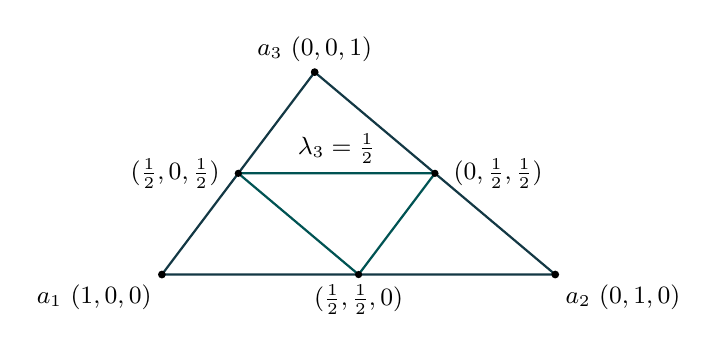
\begin{tikzpicture}[scale=0.97,thick,every node/.style={font=\small}]
\coordinate (a1) at (0,0);
\coordinate (a2) at (5.15,0);
\coordinate (a3) at (2.0,2.65);
\coordinate (m12) at ($(a1)!.5!(a2)$);
\coordinate (m13) at ($(a1)!.5!(a3)$);
\coordinate (m23) at ($(a2)!.5!(a3)$);
\draw[Heading] (a1)--(a2)--(a3)--cycle;
\draw[teal!65!black] (m12)--(m13)--(m23)--cycle;
\fill (a1) circle (1.45pt) node[below left] {\(a_1\ (1,0,0)\)};
\fill (a2) circle (1.45pt) node[below right] {\(a_2\ (0,1,0)\)};
\fill (a3) circle (1.45pt) node[above] {\(a_3\ (0,0,1)\)};
\fill (m12) circle (1.35pt) node[below] {\((\tfrac12,\tfrac12,0)\)};
\fill (m13) circle (1.35pt) node[left=3pt] {\((\tfrac12,0,\tfrac12)\)};
\fill (m23) circle (1.35pt) node[right=3pt] {\((0,\tfrac12,\tfrac12)\)};
\node[above] at ($(m13)!.5!(m23)$) {\(\lambda_3=\tfrac12\)};
\end{tikzpicture}
\par\smallskip{\small Barycentric coordinates at the vertices and edge midpoints.}
\end{center}

\subsection{Local interpolation and global nodal basis}

The three functions \(\lambda_1,\lambda_2,\lambda_3\) form a nodal basis
for \(P_1(T)\). In fact, if \(\sum_i c_i\lambda_i=0\), evaluation at
\(a_j\) gives \(c_j=0\). Since \(\dim P_1(T)=3\), they span the space.
The coefficients of any \(p\in P_1(T)\) are its vertex values.
\[
 p(x)=\sum_{i=1}^3 p(a_i)\lambda_i(x).
\]
The local degrees of freedom \(\Sigma_T\) are the three evaluation
functionals \(p\mapsto p(a_i)\).

For the reference triangle numbered \(a_1=(1,0)\), \(a_2=(0,1)\),
\(a_3=(0,0)\), the basis functions are
\(\lambda_1=x_1\), \(\lambda_2=x_2\), and
\(\lambda_3=1-x_1-x_2\).

For each interior vertex \(a_i\), construct a continuous global function
\(\phi_i\) by setting \(\phi_i(a_j)=\delta_{ij}\) at the interior vertices
and \(\phi_i=0\) at the boundary vertices. On each triangle \(T\),
\[
 \phi_i|_T=
 \begin{cases}
  \lambda_\ell^T, & a_i\text{ is local vertex }\ell\text{ of }T,\\
  0, & a_i\text{ is outside the vertex set of }T .
 \end{cases}
\]
The resulting \(\phi_i\) lie in \(C(\overline\Omega)\), restrict to
\(P_1(T)\) on each \(T\), and form a basis of \(V_h\). In particular,
\(v_h=\sum_{a_i\in\mathcal V_h^i} v_h(a_i)\phi_i\).

\subsection{Worked mesh with eight triangles}

\noindent\begin{minipage}[c]{0.65\linewidth}

The only interior vertex is \(a_5\), so \(N_d=1\). Number each
triangle counterclockwise from its right-angle vertex. Then \(a_5\)
is local vertex \(1\) on \(T_2,T_3,T_6,T_7\). Its global hat
\(\phi_5\) restricts to \(\lambda_1^{T_j}\) on those triangles and
to zero on \(T_1,T_4,T_5,T_8\).

\end{minipage}\hfill
\begin{minipage}[c]{0.32\linewidth}\centering
  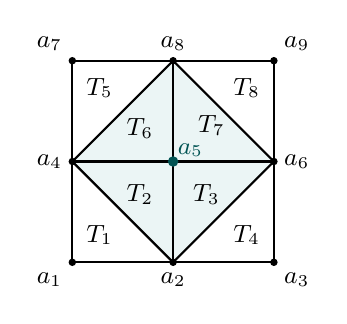
\begin{tikzpicture}[x=1.28cm,y=1.28cm,thick,every node/.style={font=\small}]
\fill[teal!8] (0,1)--(1,0)--(2,1)--(1,2)--cycle;
\draw (0,0) rectangle (2,2);
\draw (0,1)--(2,1) (1,0)--(1,2);
\draw (0,1)--(1,0)--(2,1)--(1,2)--cycle;
\foreach \x/\y/\i/\s in {0/0/1/below left,1/0/2/below,2/0/3/below right,0/1/4/left,2/1/6/right,0/2/7/above left,1/2/8/above,2/2/9/above right}{
  \fill (\x,\y) circle (1.35pt) node[\s] {\(a_{\i}\)};
}
\fill[teal!65!black] (1,1) circle (1.9pt) node[above right,inner sep=1.3pt] {\(a_5\)};
\foreach \x/\y/\j in {.27/.27/1,.67/.67/2,1.33/.67/3,1.73/.27/4,.27/1.73/5,.67/1.33/6,1.38/1.36/7,1.73/1.73/8}{
  \node at (\x,\y) {\(T_{\j}\)};
}
\end{tikzpicture}
\end{minipage}

\clearpage
\section{Lecture 14. Assembly and quadratic triangle elements}
\lecturesource{Source \enspace\texttt{Lec14.pdf}, pp.~1--8}
\label{sec:mtl781-lec14}

\subsection{The conforming linear space and its nodal basis}

Let \(\mathcal T_h\) be a triangulation of \(\Omega\subset\mathbb R^2\) and write \(P_k(T)\) for polynomials of total degree at most \(k\) on \(T\). For the homogeneous Dirichlet problem, the conforming piecewise-linear space is
\[
 V_h=\{v_h\in C(\overline\Omega)\mid
              v_h|_T\in P_1(T)\ \forall T\in\mathcal T_h,\quad
              v_h|_{\partial\Omega}=0\}.
\]
This is a subspace of \(H_0^1(\Omega)\). The dimension \(N_d=\dim V_h\) is the number of interior vertices.

For assembly we first use the full continuous piecewise-linear space, with one basis function \(\phi_i\) per mesh vertex \(a_i\). The requirements are
\[
 \phi_i(a_j)=\delta_{ij},\qquad
 \phi_i\in C(\overline\Omega),\qquad
 \phi_i|_T\in P_1(T)\quad(T\in\mathcal T_h).
\]
If the ordered local vertices of \(T\) are \(b_1,b_2,b_3\), let \(\lambda_r^T\) denote the barycentric coordinate at \(b_r\). Define \(\phi_i|_T=\lambda_r^T\) when \(a_i=b_r\) and set \(\phi_i|_T=0\) when \(a_i\) is absent from \(T\). Along any shared edge both traces are affine and take the same two endpoint values. This proves continuity and gives
\[
 \operatorname{supp}\phi_i
   =\bigcup\{T\in\mathcal T_h\mid a_i\text{ is a vertex of }T\}.
\]
The functions belonging to interior vertices form the canonical basis of \(V_h\).

\subsection{Assembly on the nine-vertex mesh}

\begin{center}
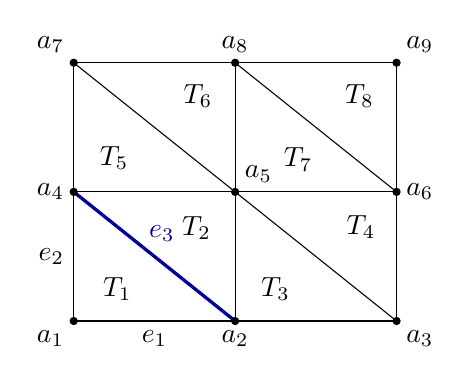
\begin{tikzpicture}[x=2.05cm,y=1.64cm]
  \draw (0,0) rectangle (2,2);
  \draw (0,1)--(2,1) (1,0)--(1,2);
  \draw (0,1)--(1,0) (1,1)--(2,0) (0,2)--(1,1) (1,2)--(2,1);
  \draw[very thick,blue!60!black] (0,1)--(1,0);
  \foreach \x/\y/\i/\pos in {0/0/1/below left,1/0/2/below,2/0/3/below right,
    0/1/4/left,1/1/5/above right,2/1/6/right,
    0/2/7/above left,1/2/8/above,2/2/9/above right}
    {\fill (\x,\y) circle (1.5pt) node[\pos] {$a_{\i}$};}
  \foreach \x/\y/\i in {.27/.25/1,.76/.72/2,1.25/.25/3,1.78/.73/4,
      .25/1.26/5,.77/1.74/6,1.39/1.25/7,1.77/1.74/8}
    {\node at (\x,\y) {$T_{\i}$};}
  \node[below] at (.5,0) {$e_1$};
  \node[left] at (0,.5) {$e_2$};
  \node[blue!60!black,above right,inner sep=2pt] at (.43,.57) {$e_3$};
\end{tikzpicture}
\end{center}
The ordered vertices of each triangle specify its local barycentric coordinates.
\[
\begin{array}{c|cccc}
T & T_1&T_2&T_3&T_4\\
\text{local vertex indices}&(1,2,4)&(5,4,2)&(2,3,5)&(6,5,3)\\[3pt]
T & T_5&T_6&T_7&T_8\\
\text{local vertex indices}&(4,5,7)&(8,7,5)&(5,6,8)&(9,8,6)
\end{array}
\]
The restrictions of all nine basis functions are listed below. Every restriction omitted from the table is zero.

\begin{center}
\begin{tabular}{c l}
\toprule
Basis function & Nonzero local restrictions \\
\midrule
\(\phi_1\) & \(\lambda_1^{T_1}\) \\
\(\phi_2\) & \(\lambda_2^{T_1},\,\lambda_3^{T_2},\,\lambda_1^{T_3}\) \\
\(\phi_3\) & \(\lambda_2^{T_3},\,\lambda_3^{T_4}\) \\
\(\phi_4\) & \(\lambda_3^{T_1},\,\lambda_2^{T_2},\,\lambda_1^{T_5}\) \\
\(\phi_5\) & \(\lambda_1^{T_2},\,\lambda_3^{T_3},\,\lambda_2^{T_4},\,
              \lambda_2^{T_5},\,\lambda_3^{T_6},\,\lambda_1^{T_7}\) \\
\(\phi_6\) & \(\lambda_1^{T_4},\,\lambda_2^{T_7},\,\lambda_3^{T_8}\) \\
\(\phi_7\) & \(\lambda_3^{T_5},\,\lambda_2^{T_6}\) \\
\(\phi_8\) & \(\lambda_1^{T_6},\,\lambda_3^{T_7},\,\lambda_2^{T_8}\) \\
\(\phi_9\) & \(\lambda_1^{T_8}\) \\
\bottomrule
\end{tabular}
\end{center}

The edge \(e_3\) joins \(a_2\) and \(a_4\) and is shared by \(T_1\) and \(T_2\). The two traces of \(\phi_1\) are zero at both \(a_2\) and \(a_4\), so both are identically zero along \(e_3\). The same endpoint argument applies to every shared edge and each \(\phi_i\).
The lecture leaves \(\phi_6,\phi_7,\phi_9\) as exercises. Their restrictions follow by locating the corresponding vertex in the local ordering above.

\smallskip
The full matrix and load vector have sizes \(9\times9\) and \(9\times1\), respectively. With the symmetric bilinear form \(a\), their entries are
\[
 \widetilde A_{ij}=a(\phi_i,\phi_j),
 \qquad \widetilde F_i=\ell(\phi_i)
 \qquad (1\leq i,j\leq9).
\]
The Dirichlet nodes are \(a_1,a_2,a_3,a_4,a_6,a_7,a_8,a_9\). Free nodes are the full set of nodes with the Dirichlet nodes removed. Here the free set consists only of \(a_5\).
Let \(I\) contain the free indices and \(D\) the Dirichlet indices. For homogeneous Dirichlet data, set \(U_D=0\) and solve
\[
 \widetilde A_{II} U_I=\widetilde F_I.
\]
Here this is the scalar equation \(a(\phi_5,\phi_5)U_5=\ell(\phi_5)\).
With prescribed values \(U_D\), the right-hand side would be \(\widetilde F_I-\widetilde A_{ID}U_D\). The free-node formula in the handwritten notes has the factors in the wrong order. In matrix notation the homogeneous solution is \(U_I=\widetilde A_{II}^{-1}\widetilde F_I\) when the free block is invertible.

For the diffusion form, the stiffness entries assemble element by element,
\[
 a(\phi_i,\phi_j)=\int_\Omega\nabla\phi_i\cdot\nabla\phi_j\,dx
   =\sum_{T\in\mathcal T_h}\int_T\nabla\phi_i\cdot\nabla\phi_j\,dx.
\]
If \(a_i\) and \(a_j\) share no triangle, each integrand vanishes on the interior of the corresponding element. This accounts for the sparsity of the stiffness matrix. For example, \(\widetilde A_{19}=0\).

\paragraph{Exercise on positive definiteness.}
For a coefficient vector \(z\) indexed by the free nodes, set \(w_h=\sum_{i\in I}z_i\phi_i\). Then
\[
 z^{\mathsf T}\widetilde A_{II}z=a(w_h,w_h)
    =\int_\Omega|\nabla w_h|^2\,dx .
\]
For \(z\ne0\), the nodal property gives \(w_h\ne0\), so the energy is positive by the zero trace and Poincaré's inequality. The positive-definiteness claim in the lecture applies to the Dirichlet-reduced matrix. The full diffusion matrix has the constant nodal vector in its kernel.

\subsection{A second assembly example}

\begin{center}
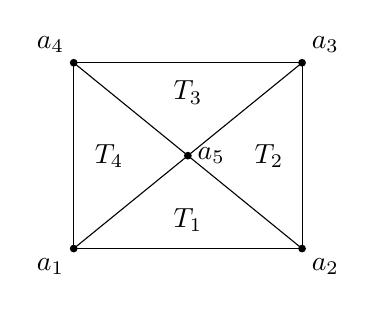
\begin{tikzpicture}[x=1.45cm,y=1.18cm]
  \draw (0,0) rectangle (2,2);
  \draw (0,0)--(2,2) (0,2)--(2,0);
  \foreach \x/\y/\i/\pos in {0/0/1/below left,2/0/2/below right,
    2/2/3/above right,0/2/4/above left,1/1/5/right}
    {\fill (\x,\y) circle (1.4pt) node[\pos] {$a_{\i}$};}
  \node at (1,.31) {$T_1$};
  \node at (1.71,1) {$T_2$};
  \node at (1,1.68) {$T_3$};
  \node at (.31,1) {$T_4$};
\end{tikzpicture}
\end{center}
We take the local orders
\[
 T_1:(a_5,a_1,a_2),\quad T_2:(a_5,a_2,a_3),\quad
 T_3:(a_5,a_3,a_4),\quad T_4:(a_5,a_4,a_1).
\]
These orders retain the labels shown in the sketch and complete the unspecified labels. The full matrix is \(5\times5\). The first and central basis functions are
\[
 \phi_1|_T=\begin{cases}
  \lambda_2^{T_1} & T=T_1,\\
  \lambda_3^{T_4} & T=T_4,\\
  0 & \text{otherwise},
 \end{cases}
 \qquad
 \phi_5|_{T_r}=\lambda_1^{T_r}\qquad(1\leq r\leq4).
\]
\textit{Exercise.} Write down \(\phi_2,\phi_3,\phi_4\). With these local orders, their nonzero pieces are
\[
\begin{array}{c|ccc}
 &\phi_2&\phi_3&\phi_4\\
\hline
 &\lambda_3^{T_1},\,\lambda_2^{T_2}
 &\lambda_3^{T_2},\,\lambda_2^{T_3}
 &\lambda_3^{T_3},\,\lambda_2^{T_4}
\end{array}
\]
and the only free vertex is \(a_5\).

\subsection{The local Lagrange element of degree one}

Let a triangle \(T\) have vertices \(a_1,a_2,a_3\) and barycentric coordinates \(\lambda_1,\lambda_2,\lambda_3\). Thus
\[
 x=\sum_{i=1}^3\lambda_i(x)a_i,\qquad \sum_{i=1}^3\lambda_i(x)=1 .
\]
Every \(p\in P_1(T)\) is determined by its values at the three vertices,
\[
 p(x)=\sum_{i=1}^3 p(a_i)\lambda_i(x).
\]
The degree-one Lagrange element is the triple \((T,P_1(T),\Sigma_T)\), where \(\Sigma_T=\{p\mapsto p(a_i)\mid 1\le i\le 3\}\) is its set of degrees of freedom. Its local node set can be written as
\[
 L_1(T)=\{x\in T\mid \lambda_i(x)\in\{0,1\}\text{ for every }i\}
       =\{a_1,a_2,a_3\}.
\]

\subsection{The conforming quadratic approximation}

For the two-dimensional homogeneous Dirichlet problem with the reaction term shown in the lecture, find \(u\in H_0^1(\Omega)\) with
\[
 \underbrace{\int_\Omega\nabla u\cdot\nabla v\,dx+
             \int_\Omega uv\,dx}_{a(u,v)}
   =\underbrace{\int_\Omega fv\,dx}_{\ell(v)}
   \qquad (v\in H_0^1(\Omega)).
\]
Its quadratic finite element approximation uses
\[
 V_h=\{v_h\in C(\overline\Omega)\mid
     v_h|_T\in P_2(T)\ \forall T\in\mathcal T_h,\quad
     v_h|_{\partial\Omega}=0\}\subset H_0^1(\Omega).
\]
Find \(u_h\in V_h\) such that \(a(u_h,v_h)=\ell(v_h)\) for every \(v_h\in V_h\). The discrete problem is well posed because \(a(v_h,v_h)=\|v_h\|_{H^1(\Omega)}^2\). For a basis \(\{\psi_i\}_{i=1}^{N_d}\) of \(V_h\), let \(u_h=\sum_{i=1}^{N_d}\alpha_i\psi_i\), where \(N_d=\dim V_h\). Testing with the basis functions gives \(AU=F\) with
\[
 A_{ij}=a(\psi_j,\psi_i)=a(\psi_i,\psi_j),\qquad
 F_i=\ell(\psi_i),\qquad U_i=\alpha_i
 \qquad(1\leq i,j\leq N_d).
\]

\subsection{The local Lagrange element of degree two}

The space \(P_2(T)\) has dimension \(6\). Use its three vertices and three edge midpoints as nodes, writing
\[
 a_{ij}=\frac{a_i+a_j}{2}\quad(1\leq i<j\leq3),\qquad
 m_1=a_{23},\quad m_2=a_{13},\quad m_3=a_{12}.
\]
In barycentric coordinates \(m_1=(0,\tfrac12,\tfrac12)\), with the other two obtained by permuting the coordinates.

\begin{center}
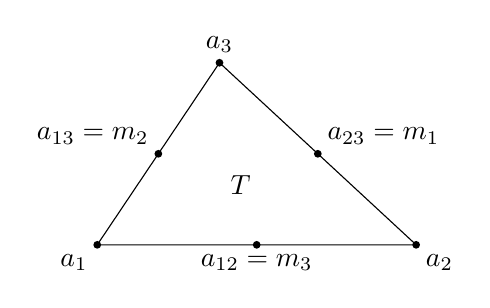
\begin{tikzpicture}[x=1.35cm,y=1.25cm]
  \draw (0,0)--(3,0)--(1.15,1.85)--cycle;
  \node at (1.35,.61) {$T$};
  \fill (0,0) circle (1.4pt) node[below left] {$a_1$};
  \fill (3,0) circle (1.4pt) node[below right] {$a_2$};
  \fill (1.15,1.85) circle (1.4pt) node[above] {$a_3$};
  \fill (2.075,.925) circle (1.4pt) node[above right] {$a_{23}=m_1$};
  \fill (.575,.925) circle (1.4pt) node[above left] {$a_{13}=m_2$};
  \fill (1.5,0) circle (1.4pt) node[below] {$a_{12}=m_3$};
\end{tikzpicture}
\end{center}

Construct the six cardinal polynomials with the following values for \(1\le i,j\le3\),
\[
 \phi^{a_i}(a_j)=\delta_{ij},\quad \phi^{a_i}(m_j)=0,\qquad
 \phi^{m_i}(a_j)=0,\quad \phi^{m_i}(m_j)=\delta_{ij}.
\]
The formulas in terms of the local barycentric coordinates are
\begin{align*}
 \phi^{a_i}(x)&=2\lambda_i(x)\bigl(\lambda_i(x)-\tfrac12\bigr)
               =\lambda_i(x)\bigl(2\lambda_i(x)-1\bigr),\\
 \phi^{m_1}(x)&=4\lambda_2(x)\lambda_3(x),\\
 \phi^{m_2}(x)&=4\lambda_1(x)\lambda_3(x),\\
 \phi^{m_3}(x)&=4\lambda_1(x)\lambda_2(x).
\end{align*}
At a vertex, one barycentric coordinate is one and the rest are zero. At a midpoint, two coordinates are \(\tfrac12\) and the remaining one is zero. These give the required nodal values. The resulting functions are linearly independent by evaluation at the nodes and form the canonical basis by \(\dim P_2(T)=6\). For \(p\in P_2(T)\), the coefficients of the basis expansion are \(p(a_i)\) and \(p(m_i)\), so
\[
 p(x)=\sum_{i=1}^3 p(a_i)\phi^{a_i}(x)
       +\sum_{i=1}^3 p(m_i)\phi^{m_i}(x).
\]
The element is \((T,P_2(T),\Sigma_T)\), where
\[
 \Sigma_T=\{p\mapsto p(a_i),\ p\mapsto p(m_i)\mid 1\le i\le3\}.
\]
Equivalently the degrees of freedom evaluate \(p\) at the nodes
\[
 L_2(T)=\{x\in T\mid \lambda_i(x)\in\{0,\tfrac12,1\}
                          \text{ for every }i\}
       =\{a_1,a_2,a_3,m_1,m_2,m_3\}.
\]
Thus the values on \(L_2(T)\) determine every polynomial in \(P_2(T)\) uniquely.

\clearpage
\section{Lecture 15. Lagrange elements and the finite element error estimate}
\lecturesource{Source \enspace\texttt{Lec15\_annotated.pdf}, pp.~1--11}
\label{sec:mtl781-lec15}

\subsection{Assembling the conforming quadratic space}

On the triangle \(T\), let \(\lambda_i\) be the barycentric coordinates and \(a_{ij}=(a_i+a_j)/2\) for \(i<j\). The degree-two Lagrange element \((T,P_2(T),\Sigma_2(T))\) uses point evaluations at
\[
 L_2(T)=\{x\in T\mid \lambda_i(x)\in\{0,\tfrac12,1\}
                              \text{ for every }i\}.
\]
The six evaluations comprise \(\{p\mapsto p(a_i)\}_{i=1}^3\) and \(\{p\mapsto p(a_{ij})\}_{i<j}\). The local expansion is
\[
 p(x)=\sum_{i=1}^3\lambda_i(x)\bigl(2\lambda_i(x)-1\bigr)p(a_i)
          +\sum_{1\leq i<j\leq3}4\lambda_i(x)\lambda_j(x)p(a_{ij}).
\]

Let \(\mathcal V_h\) and \(\mathcal E_h\) be the sets of mesh vertices and edges. For the full space
\[
 \widetilde V_h=\{v_h\in C(\overline\Omega)\mid
                  v_h|_T\in P_2(T)\ \forall T\in\mathcal T_h\},
\]
there is one nodal degree of freedom for each vertex and each edge midpoint. Indeed adjacent elements agree along an edge whenever they match at its two endpoints and midpoint, since a polynomial of degree at most two on that edge is determined by those three values. Therefore
\[
 \dim\widetilde V_h=|\mathcal V_h|+|\mathcal E_h|.
\]
Write \(\mathcal V_h^b\) for the boundary vertices and \(\mathcal M_h^b\) for the set of midpoints of boundary edges. The same three-point argument gives
\[
 v_h|_{\partial\Omega}=0
 \quad\Longleftrightarrow\quad
 v_h(p)=0\quad\text{for every }p\in\mathcal V_h^b\cup\mathcal M_h^b.
\]
The dimension of the homogeneous Dirichlet space \(V_h\) is \(|\mathcal V_h^i|+|\mathcal E_h^i|\), with superscript \(i\) denoting interior vertices or interior edges.

\paragraph{A square split into two triangles.}
The local vertex orders are \(T_1:(a_1,a_2,a_3)\) and \(T_2:(a_4,a_3,a_2)\). Use \(\phi_i\) for the basis function at vertex \(a_i\) and \(\psi_i\) for the one at midpoint \(m_i\). Both triangles contain \(m_5\).

\begin{center}
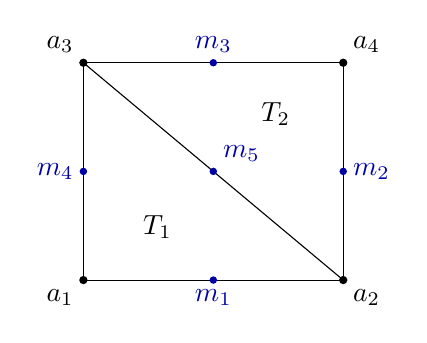
\begin{tikzpicture}[x=1.65cm,y=1.38cm]
  \draw (0,0) rectangle (2,2);
  \draw (0,2)--(2,0);
  \foreach \x/\y/\i/\pos in {0/0/1/below left,2/0/2/below right,
                          0/2/3/above left,2/2/4/above right}
    {\fill (\x,\y) circle (1.5pt) node[\pos] {$a_{\i}$};}
  \foreach \x/\y/\i/\pos in {1/0/1/below,2/1/2/right,1/2/3/above,
                          0/1/4/left,1/1/5/above right}
    {\fill[blue!65!black] (\x,\y) circle (1.35pt) node[\pos] {$m_{\i}$};}
  \node at (.57,.49) {$T_1$};
  \node at (1.48,1.53) {$T_2$};
\end{tikzpicture}
\end{center}

For concision put \(q(s)=s(2s-1)\). Three of the basis functions from the lecture are
\[
\begin{array}{c|cc}
 &T_1&T_2\\\hline
 \phi_1&q(\lambda_1^{T_1})&0\\
 \phi_2&q(\lambda_2^{T_1})&q(\lambda_3^{T_2})\\
 \psi_5&4\lambda_2^{T_1}\lambda_3^{T_1}
        &4\lambda_2^{T_2}\lambda_3^{T_2}
\end{array}
\]
\textit{Exercise.} Write down the remaining basis functions. Applying the same local formulas gives
\[
\begin{array}{c|cc}
 &T_1&T_2\\\hline
 \phi_3&q(\lambda_3^{T_1})&q(\lambda_2^{T_2})\\
 \phi_4&0&q(\lambda_1^{T_2})\\
 \psi_1&4\lambda_1^{T_1}\lambda_2^{T_1}&0\\
 \psi_2&0&4\lambda_1^{T_2}\lambda_3^{T_2}\\
 \psi_3&0&4\lambda_1^{T_2}\lambda_2^{T_2}\\
 \psi_4&4\lambda_1^{T_1}\lambda_3^{T_1}&0
\end{array}
\]
The full space has dimension \(4+5=9\). Only \(m_5\) is free for homogeneous Dirichlet data, so its basis function spans \(V_h\) on this mesh.

\subsection{The cubic and general Lagrange elements}

The local cubic space has dimension \(\dim P_3(T)=10\). In addition to \(a_1,a_2,a_3\), take the six edge nodes
\[
 a_{iij}=\frac{2a_i+a_j}{3}\qquad (1\leq i,j\leq3,\ i\ne j)
\]
and the centroid
\[
 a_{123}=\frac{a_1+a_2+a_3}{3}.
\]
The formula \(a_{ijk}=(a_i+a_j+a_k)/3\) for \(1\leq i<j<k\leq3\) consequently gives only \(a_{123}\). The repeated index of \(a_{iij}\) indicates the closer vertex.

\begin{center}
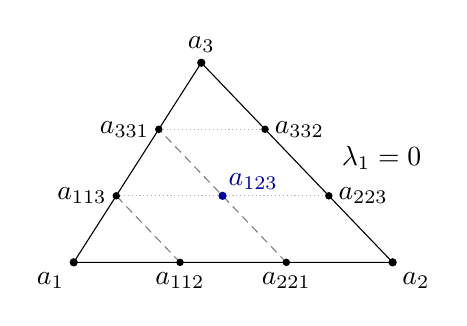
\begin{tikzpicture}[x=1.35cm,y=1.3cm]
  \draw (0,0)--(3,0)--(1.2,1.95)--cycle;
  \draw[gray!60,densely dotted] (.4,.65)--(2.4,.65) (.8,1.3)--(1.8,1.3);
  \draw[gray,densely dashed] (1,0)--(.4,.65) (2,0)--(.8,1.3);
  \fill (0,0) circle (1.5pt) node[below left] {$a_1$};
  \fill (3,0) circle (1.5pt) node[below right] {$a_2$};
  \fill (1.2,1.95) circle (1.5pt) node[above] {$a_3$};
  \fill (1,0) circle (1.35pt) node[below] {$a_{112}$};
  \fill (2,0) circle (1.35pt) node[below] {$a_{221}$};
  \fill (.4,.65) circle (1.35pt) node[left] {$a_{113}$};
  \fill (.8,1.3) circle (1.35pt) node[left] {$a_{331}$};
  \fill (2.4,.65) circle (1.35pt) node[right] {$a_{223}$};
  \fill (1.8,1.3) circle (1.35pt) node[right] {$a_{332}$};
  \fill[blue!65!black] (1.4,.65) circle (1.5pt)
    node[above right,inner sep=2pt] {$a_{123}$};
  \node[right] at (2.43,1.02) {$\lambda_1=0$};
\end{tikzpicture}
\end{center}
The dashed segments parallel to the edge \([a_2,a_3]\) are the levels \(\lambda_1=\tfrac23\) and \(\lambda_1=\tfrac13\).

Each cardinal polynomial equals one at its named node and zero at the other nine nodes. For example, \(\phi^{a_i}(a_j)=\delta_{ij}\) and \(\phi^{a_i}\) vanishes at all edge nodes and at \(a_{123}\). The first vertex function is
\[
 \phi^{a_1}(x)=\frac92\lambda_1\bigl(\lambda_1-\tfrac13\bigr)
                           \bigl(\lambda_1-\tfrac23\bigr).
\]
For all vertices, edge nodes and the centroid the formulas are
\begin{align*}
 \phi^{a_i}(x)
  &=\tfrac12\lambda_i(3\lambda_i-1)(3\lambda_i-2),\\
 \phi^{a_{iij}}(x)
  &=\tfrac{27}{2}\lambda_i\lambda_j\bigl(\lambda_i-\tfrac13\bigr)
   =\tfrac92\lambda_i\lambda_j(3\lambda_i-1)
    \qquad(i\ne j),\\
 \phi^{a_{123}}(x)&=27\lambda_1\lambda_2\lambda_3 .
\end{align*}
In particular, the \(a_{112}\) polynomial is \(\tfrac92\lambda_1\lambda_2(3\lambda_1-1)\). At \(a_{iij}\) the two nonzero coordinates are \(\lambda_i=\tfrac23\) and \(\lambda_j=\tfrac13\). At \(a_{123}\) all three are \(\tfrac13\). These values, together with the vertex coordinates, verify the cardinal property. The ten functions are independent by evaluation, so they form a basis. For \(p\in P_3(T)\) the nodal expansion becomes
\begin{align*}
 p(x)
 &=\tfrac12\sum_{i=1}^3\lambda_i(3\lambda_i-1)(3\lambda_i-2)\,p(a_i)\\
 &\quad+\tfrac92\sum_{\substack{1\leq i,j\leq3\\i\ne j}}
      \lambda_i\lambda_j(3\lambda_i-1)\,p(a_{iij})\\
 &\quad+27\lambda_1\lambda_2\lambda_3\,p(a_{123}).
\end{align*}
The nodal set is
\[
 L_3(T)=\{x\in T\mid\lambda_i(x)\in\{0,\tfrac13,\tfrac23,1\}
                                \text{ for every }i\}.
\]
The corresponding degrees of freedom are \(\Sigma_3(T)=\{p\mapsto p(x)\mid x\in L_3(T)\}\), giving the element \((T,P_3(T),\Sigma_3(T))\). In the cubic formulas, the values at edge nodes use the repeated indices \(a_{iij}\). The notation \(a_{ij}\) in the handwritten list would refer to a quadratic edge midpoint.

For any \(k\geq1\) the degree-\(k\) element is \((T,P_k(T),\Sigma_k(T))\), where
\begin{align*}
 L_k(T)
  &=\left\{x=\sum_{i=1}^3\lambda_i a_i\ \middle|\
       \sum_{i=1}^3\lambda_i=1,\ 
       \lambda_i\in\{0,\tfrac1k,\tfrac2k,\ldots,1\}
       \text{ for every }i\right\},\\
 \Sigma_k(T)&=\{p\mapsto p(x)\mid x\in L_k(T)\}.
\end{align*}
The nodes correspond to nonnegative integer triples with entries summing to \(k\), so their number is \(\binom{k+2}{2}=\dim P_k(T)\).

\subsection{Céa's lemma}

A boundary-value problem gives a weak solution \(u\) and then a finite element solution \(u_h\). Let \(V\) be the Hilbert space of the weak formulation and \(V_h\subset V\) the conforming finite element space. The two problems are to find
\begin{align}
 u\in V&\quad\text{such that}\quad a(u,v)=\ell(v)
       &&(v\in V),\label{eq:781-l15-weak}\\
 u_h\in V_h&\quad\text{such that}\quad a(u_h,v_h)=\ell(v_h)
       &&(v_h\in V_h).\label{eq:781-l15-discrete}
\end{align}
Assume \(a\) is continuous and \(V\)-elliptic (coercive), so that for constants \(M,\alpha>0\),
\[
 |a(w,v)|\le M\|w\|_V\|v\|_V,\qquad
 a(v,v)\ge \alpha\|v\|_V^2\qquad(w,v\in V).
\]
Together with a continuous load \(\ell\), these hypotheses give well-posed problems. For the Dirichlet example, take \(V=H_0^1(\Omega)\) with the \(H^1\) norm, as used in the later estimates. The \(H^1\) seminorm also defines an equivalent norm on this space by Poincaré's inequality.

\paragraph{Céa's lemma.}
For the solutions \(u\) and \(u_h\) the error obeys
\[
 \|u-u_h\|_V\le \frac{M}{\alpha}
                      \inf_{v_h\in V_h}\|u-v_h\|_V.
\]
\begin{proof}
Since \(V_h\subset V\), the continuous equation can be tested with any \(v_h\in V_h\). Subtracting the discrete equation gives Galerkin orthogonality,
\[
 a(u-u_h,v_h)=0 \qquad(v_h\in V_h).
\]
Write \(e=u-u_h\). For an arbitrary \(v_h\in V_h\), \(v_h-u_h\) lies in \(V_h\), so
\begin{align*}
 \alpha\|e\|_V^2
 &\le a(e,e)\\
 &=a(e,u-v_h)+a(e,v_h-u_h)\\
 &=a(e,u-v_h)
 \le M\|e\|_V\|u-v_h\|_V .
\end{align*}
If \(\|e\|_V=0\) the bound holds immediately. Otherwise divide by \(\alpha\|e\|_V\) and take the infimum over \(V_h\).
\end{proof}
When the nodal interpolant \(\Pi_hu\) is defined and belongs to \(V_h\), the choice \(v_h=\Pi_hu\) gives
\[
 \|u-u_h\|_V\le \frac{M}{\alpha}\|u-\Pi_hu\|_V .
\]
This reduces the estimate of the Galerkin error to that of the interpolation error.

\subsection{The one-dimensional Dirichlet problem and its interpolant}

On \(\Omega=(0,1)\), consider
\[
 -\bigl(a(x)u'(x)\bigr)'=f(x),\qquad u(0)=u(1)=0,\qquad
 f\in L^2(0,1).
\]
Assume \(a(x)\) is bounded and bounded below by a positive constant so that the diffusion form is continuous and coercive. The weak problem is to find \(u\in H_0^1(0,1)\) satisfying
\[
 a(u,v)=\int_0^1 a(x)u'(x)v'(x)\,dx
    =\int_0^1 f(x)v(x)\,dx=\ell(v)
   \qquad(v\in H_0^1(0,1)).
\]

Partition \([0,1]\) by \(0=x_0<x_1<\cdots<x_N=1\), and set \(I_j=[x_{j-1},x_j]\), \(h_j=x_j-x_{j-1}\) and \(h=\max_{1\leq j\leq N}h_j\). Here \(N\) is the number of subintervals. This convention reconciles the two different uses of \(N\) in the lecture's mesh sketches. Define
\[
 V_h=\{v_h\in C([0,1])\mid v_h|_{I_j}\in P_1(I_j)\
              (1\leq j\leq N),\quad v_h(0)=v_h(1)=0\}.
\]
The conforming approximation is \(u_h\in V_h\) with \(a(u_h,v_h)=\ell(v_h)\) for every \(v_h\in V_h\). By Céa's lemma,
\[
 \|u-u_h\|_{H^1(0,1)}\le \frac M\alpha\|u-v_h\|_{H^1(0,1)}
 \qquad(v_h\in V_h).
\]

Let \(\phi_i\) be the piecewise-linear nodal hat at \(x_i\) for \(1\leq i\leq N-1\). A function \(v_h\in V_h\) has coefficients \(\alpha_i=v_h(x_i)\) in this basis. In one dimension a function \(v\in H_0^1(0,1)\) has a continuous representative. The nodal interpolation operator \(\Pi_h:H_0^1(0,1)\to V_h\) is therefore given by
\[
 \Pi_h v=\sum_{i=1}^{N-1} v(x_i)\phi_i,\qquad
 (\Pi_h v)(x_i)=v(x_i)\quad(0\leq i\leq N).
\]

\begin{center}
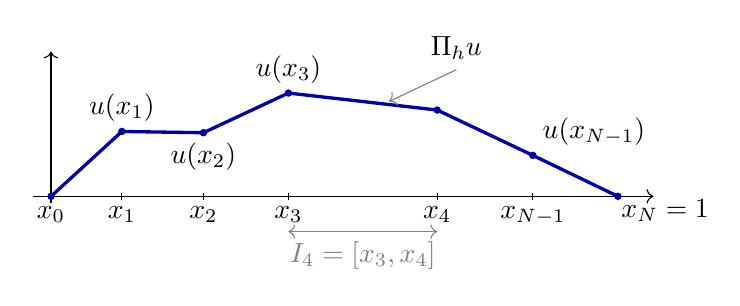
\begin{tikzpicture}[x=.9cm,y=.8cm]
  \draw[->] (-.25,0)--(8.5,0);
  \draw[->] (0,-.1)--(0,2.3);
  \draw[very thick,blue!65!black]
    (0,0)--(1,1.03)--(2.15,1.01)--(3.35,1.64)--(5.45,1.37)--(6.8,.65)--(8,0);
  \foreach \x/\y in {0/0,1/1.03,2.15/1.01,3.35/1.64,5.45/1.37,6.8/.65,8/0}{
    \draw (\x,.06)--(\x,-.06);
    \fill[blue!65!black] (\x,\y) circle (1.35pt);
  }
  \node[below] at (0,0) {$x_0$};
  \node[below] at (1,0) {$x_1$};
  \node[below] at (2.15,0) {$x_2$};
  \node[below] at (3.35,0) {$x_3$};
  \node[below] at (6.8,0) {$x_{N-1}$};
  \node[below right,inner sep=1pt] at (8,0) {$x_N=1$};
  \node[below] at (5.45,0) {$x_4$};
  \draw[gray,<->] (3.35,-.56)--(5.45,-.56)
    node[midway,below] {$I_4=[x_3,x_4]$};
  \node[above] at (1,1.03) {$u(x_1)$};
  \node[below] at (2.15,1.01) {$u(x_2)$};
  \node[above] at (3.35,1.64) {$u(x_3)$};
  \node[above right] at (6.8,.65) {$u(x_{N-1})$};
  \draw[gray,->,shorten >=2pt] (5.72,2.01)--(4.7,1.47);
  \node[above] at (5.72,2.01) {$\Pi_hu$};
\end{tikzpicture}
\end{center}

In one dimension \(H^1(0,1)\hookrightarrow C([0,1])\) and \(H^2(0,1)\hookrightarrow C^1([0,1])\). For the two-dimensional polygonal domains of the triangular example, \(H^2(\Omega)\hookrightarrow C(\overline\Omega)\), whereas \(H^1(\Omega)\) alone need not supply a continuous representative for nodal evaluation.

\subsection{Interpolation error for piecewise-linear elements}

Assume \(u\in H^2(0,1)\cap H_0^1(0,1)\) and let \(u_I=\Pi_hu\). Set \(e_I=u-u_I\) and recall the norm decomposition
\[
 \|e_I\|_{H^1(0,1)}^2
     =\|e_I\|_{L^2(0,1)}^2+|e_I|_{H^1(0,1)}^2.
\]

\paragraph{Derivative estimate.}
On \(I_j=[x_{j-1},x_j]\) the interpolant has constant slope
\[
 u_I'(x)=\frac{u(x_j)-u(x_{j-1})}{h_j}.
\]
Since \(u\) has a \(C^1\) representative, the mean value theorem supplies \(\xi_j\in(x_{j-1},x_j)\) with \(u'(\xi_j)=u_I'|_{I_j}\). The function \(u'\) has an absolutely continuous representative with derivative \(u''\), so for \(x\) in the interior of \(I_j\)
\begin{align}
 |u'(x)-u_I'(x)|
 &=\left|\int_{\xi_j}^x u''(t)\,dt\right|\notag\\
 &\le |x-\xi_j|^{1/2}
       \left(\int_{I_j}|u''(t)|^2\,dt\right)^{1/2}
 \le h_j^{1/2}\|u''\|_{L^2(I_j)}.
 \label{eq:781-l15-interp-pointwise}
\end{align}
The estimate follows by Cauchy--Schwarz on the interval between \(\xi_j\) and \(x\). Squaring and integrating on \(I_j\) gives
\[
 \int_{I_j}|u'(x)-u_I'(x)|^2\,dx
       \le h_j^2\int_{I_j}|u''(t)|^2\,dt .
\]
Summing and using \(h_j\le h\) yields
\begin{align*}
 |e_I|_{H^1(0,1)}^2
    &=\sum_{j=1}^{N}\int_{I_j}|u'(x)-u_I'(x)|^2\,dx\\
    &\le h^2\sum_{j=1}^{N}\|u''\|_{L^2(I_j)}^2
     =h^2|u|_{H^2(0,1)}^2 .
\end{align*}
Consequently \(|e_I|_{H^1(0,1)}\le h\,|u|_{H^2(0,1)}\), which is \(O(h)\) for fixed \(u\).

\pagebreak[4]
\paragraph{\(L^2\) estimate.}
Since \(e_I(x_{j-1})=0\), for \(x\in I_j\) the preceding pointwise estimate gives
\begin{align*}
 |e_I(x)|
 &=\left|\int_{x_{j-1}}^{x}(u'(s)-u_I'(s))\,ds\right|\\
 &\le \int_{x_{j-1}}^x h_j^{1/2}\|u''\|_{L^2(I_j)}\,ds
 \le h_j^{3/2}\|u''\|_{L^2(I_j)} .
\end{align*}
After squaring and integrating on \(I_j\), we obtain
\[
 \int_{I_j}|u-u_I|^2\,dx\le h_j^4\int_{I_j}|u''|^2\,dx .
\]
Summing over the mesh gives
\[
 \|e_I\|_{L^2(0,1)}^2
    \le h^4|u|_{H^2(0,1)}^2,\qquad
 \|e_I\|_{L^2(0,1)}\le h^2|u|_{H^2(0,1)} .
\]
The \(L^2\) norm of the interpolation error is \(O(h^2)\), and its square is \(O(h^4)\). The handwritten order \(O(h^2)\) next to the squared norm belongs to the norm.

\paragraph{Full \(H^1\) norm and Galerkin error.}
Combining the two estimates and using \(h\le1\) gives
\[
 \|u-u_I\|_{H^1(0,1)}^2
     \le (h^4+h^2)|u|_{H^2(0,1)}^2
     =h^2(1+h^2)|u|_{H^2(0,1)}^2
     \le 2h^2|u|_{H^2(0,1)}^2.
\]
Thus \(\|u-u_I\|_{H^1(0,1)}\le\sqrt2\,h\,|u|_{H^2(0,1)}\).
With \(v_h=u_I\), Céa's lemma gives the first-order Galerkin estimate
\[
 \boxed{\ \|u-u_h\|_{H^1(0,1)}
              \le \frac{\sqrt2\,M}{\alpha}
                       h\,|u|_{H^2(0,1)}\ } .
\]
The constant is independent of the mesh size.

\end{document}
